\documentclass{article}
\usepackage[utf8]{inputenc}
\usepackage{amsmath, amssymb, amsfonts, amsthm}
\usepackage{mathtools}
\usepackage{mdframed}
\usepackage{cancel}
\usepackage{import, xifthen, pdfpages, transparent}
\usepackage{enumitem}
\usepackage{geometry}
\usepackage{multicol}
\usepackage{hyperref}
\usepackage{float}
\usepackage{tikz, pgfplots}
\usetikzlibrary{positioning}
\pgfplotsset{compat=1.18}
\geometry{a4paper, margin=2cm}

\newmdenv[
  linecolor=black,
  linewidth=1pt,
  roundcorner=5pt,
  innertopmargin=4pt,
  innerbottommargin=10pt,
  innerleftmargin=10pt,
  innerrightmargin=10pt
]{bxthm}

\theoremstyle{plain}
\newtheorem{thm}{Teorema}[section]
\newtheorem{lem}[thm]{Lemma}
\newtheorem{prop}[thm]{Proposizione}
\newtheorem{cor}{Corollario}

\theoremstyle{definition}
\newtheorem{defn}{Definizione}[section]
\newtheorem{exmp}{Esempio}[section]
\newtheorem{xca}[exmp]{Esercizio}

\theoremstyle{remark}
\newtheorem{rem}{Osservazione}
\newtheorem{note}{Nota}
\newtheorem{case}{Caso}

\newcommand{\incfig}[2][\columnwidth]{%
    \def\svgwidth{#1}
    \import{./figures/}{#2.pdf_tex}
}

\begin{document}

\begin{titlepage}
    \centering
	{\textsc{Università degli Studi della Basilicata} \par}
	\vspace{2cm}
    {\huge\bfseries Appunti rielaborati di Analisi II 2024/2025\par}
    \vfill
	{\Large\itshape Donato Martinelli\par}
	{\large \today\par}
\end{titlepage}
%\tableofcontents

\newpage 

% \section{Applicazioni multivariabili e prodotti cartesiani di $\mathbb{R}$}
% 
% \vspace{10pt}
% 
% \paragraph{Funzione a due variabili}
% Una funzione di $2$ variabili è una un'applicazione \[f:(x,y)\mapsto f(x,y)\in\mathbb{R}.\]
% Ad esempio
% \[f(x,y)=\sqrt{x^2+y^2}\]
% 
% \vspace{10pt}
% 
% \paragraph{Funzione a tre variabili}
% Analogalmente una funzione di 3 variabili può essere vista come un'applicazione 
% \[f:(x,y,z)\mapsto f(x,y,z)\in\mathbb{R}\]
% Ad esempio
% \[f(x,y,z)=\sqrt{x^2+y^2-z}\]
% 
% \vspace{10pt}
% 
% \paragraph{Funzione a $n$ variabili}
% Più in generale una funzione di $n$ variabili è un'applicazione 
% \[f:(x_1,\ldots,x_n)\mapsto f(x_1,\ldots,x_n)\in\mathbb{R}.\]
% 
% \vspace{10pt}
% 
% Andiamo a studiare gli insiemi delle $n$-uple.
% 
% \vspace{10pt}
% 
% Nel caso $n=2$, denotiamo con $\mathbb{R}^2$ l'insieme delle coppie ordinate di numeri reali.
% Un elemento $v\in\mathbb{R}^2$ è una coppia ordinata $(x,y)$ di numeri reali dove $x$ e $y$ sono dette componenti di $v$.
% In $\mathbb{R}^2$ definiamo due operazioni di somma e prodotto.
% Definiamo la somma al seguente modo 
% \[(x,y)+(x',y')=(x+x',y+y')\in\mathbb{R}^2\]
% Definiamo il prodotto invece 
% \[\alpha(x,y)=(\alpha x, \alpha y)\in\mathbb{R}^2\]
% Vediamo che con queste operazioni, $\mathbb{R}^2$ è uno spazio vettoriale di dimensione $2$, con base canonica $E=\{e_1,e_2\}$
% formata dai vettori $e_1=(1,0)$ e $e_2=(0,1)$. 
% L'elemento neutro rispetto alla somma è la coppia $(0,0)$ che viene chiamato lo $0$ di $\mathbb{R}^2$
% Sia $(x,y)\in\mathbb{R}^2$, allora \[(x,y)+(0,0)=(x,y).\]
% L'elemento opposto invece è l'elemento che ha come componenti gli opposti di $x$ e $y$.
% Sia $(x,y)\in\mathbb{R}^2$, allora \[(x,y)+(-x,-y)=(0,0).\]
% L'esistenza dell'opposto introduce anche l'operazione della differenza che è un caso specifico della somma. 
% Si definisce infatti 
% \[(x,y)-(x',y')=(x,y)+(-(x',y'))=(x,y)+(-x',-y')=(x-x',y-y').\]
% Si può stabilire una corrispondenza biunivoca tra $\mathbb{R}^2$ e il piano ordinario mediante la seguente applicazione:
% \[\phi: v=(x,y)\in\mathbb{R}^2\mapsto p=(x,y),\] chiamiamo $x$ e $y$ rispettivamente ascissa e ordinate.
% Quest'applicazione è biunivoca perchè se $p=(x,y)$ è un punto del piano, allora 
% \[\exists!\,v\in\mathbb{R}^2\,:\;\phi(v)=p\quad\textup{con}\;v=(x,y).\]
% 
% \vspace{10pt}
% 
% Vale lo stesso discorso per $n=3$,
% \[\mathbb{R}^3=\{(x,y,z): x,y,z\in\mathbb{R}\}\]
% Andando veloci,
% \begin{itemize}
%     \item Operazione di somma:
%     \[(x,y,z)+(x',y',z')=(x+x',y+y',z+z')\in\mathbb{R}^3\]
%     \item Operazione di prodotto ($\alpha\in\mathbb{R}$):
%     \[\alpha(x,y,z)=(\alpha x,\alpha y, \alpha z)\in\mathbb{R}^3\]
%     \item $\mathbb{R}^3$ è uno spazio vettoriale di dimensione $3$ con:
%     \begin{itemize}
%         \item Base canonica \[E=\{e_1,e_2,e_3\}=\{(1,0,0),(0,1,0),(0,0,1)\}\]
%         \item Elemento neutro rispetto alla somma $(0,0,0)$ che è lo $0$ di $\mathbb{R}^3$
%         \item L'opposto di $(x,y,z)$ è $(-x,-y,-z)$
%     \end{itemize}
%     \item Possiamo definire una corrisponenza biunivoca tra $\mathbb{R}^3$ e lo spazio ordinario mediante la seguente applicazione
%     \[\phi:v=(x,y,z)\in\mathbb{R}^3\to p=(x,y,z)\in \textup{spazio}\]
%     $x,y,z$ sono rispettivamente ascissa, ordinata, e quota.
%     $\phi$ è biunivoca perchè, preso un punto $p=(x,y,z)$ dello spazio, \[\exists!v\in\mathbb{R}^3\,:\;\phi(v)=p\quad\textup{con}\;v=(x,y,z).\]
% \end{itemize}
% 
% \vspace{10pt}
% 
% Segue immediatamente la generalizzazione per un $n$-qualsiasi. 
% \[\mathbb{R}^n=\{(x_1,\ldots,x_n)\,:\;x_1\ldots,x_n\in\mathbb{R}\}\]
% Se $v\in\mathbb{R}^n$, allora 
% \[\exists\, n\;\textup{numeri reali}\,x_1,\ldots,x_n\,:\; v=(x_1,\ldots,x_n)\]
% $\forall\,i=1,\ldots,n,\;x_i$ si dice componente di $v$.
% $\mathbb{R}^n$ è uno spazio vettoriale di dimensione $n$ con base canonica \[E=\{e_1,e_2,e_3\}=\{(1,0,\ldots,0),(0,1,\ldots,0),(0,\ldots,0,1)\}.\]
% Vale stesso discorso per somma, prodotto, elemento neutro, opposto e differenza.
% 
% \vspace{10pt}
% 
% In queste strutture non ci sono proprietà di ordinamento, quantomeno non paragonabili a quelle presenti in $\mathbb{R}$. 
% 
% \vspace{10pt}
% 
% Segue ovviamente che 
% \[\mathbb{R}\thicksim \mathbb{R}^1.\]
% 
% \vspace{10pt}

\section{Topologia di $\mathbb{R}^n$}

\vspace{10pt}

Passiamo ora a introdurre dei concetti importanti per strutturare una topologia di $\mathbb{R}^n$.

\vspace{10pt}

\paragraph{Norma di una $n$-upla}
\begin{bxthm}
\begin{defn}
    Sia $\mathbf{x}=(x_1,\ldots,x_n)\in\mathbb{R}^n$. Si definisce \textbf{norma} di $\mathbf{x}$ il numero reale 
    \[\|\mathbf{x}\|=\sqrt{\sum_{i=1}^{n}x_i^2}.\]
\end{defn}
\end{bxthm}

\vspace{10pt}

\paragraph{Proprietà della norma}
\begin{bxthm}
\begin{thm}
    Sia $\mathbf{x}=(x_1,\ldots,x_n)\in\mathbb{R}^n$, allora
    \begin{itemize}
        \item $\|\mathbf{x}\|\geq0$ e $\|\mathbf{x}\|=0 \iff \mathbf{x}=\mathbf{0};$
        \item Se $\alpha\in\mathbb{R}, \|\alpha \mathbf{x}\|=|\alpha|\cdot\|\mathbf{x}\|;$
        \item Se $\mathbf{x},\mathbf{y}\in\mathbb{R}^n$, $\|\mathbf{x}+\mathbf{y}\|\leq\|\mathbf{x}\|+\|\mathbf{y}\|;$
        \item Se $\mathbf{x},\mathbf{y}\in\mathbb{R}^n$, $\|\mathbf{x}\|-\|\mathbf{y}\|\leq\|\mathbf{x}-\mathbf{y}\|.$
    \end{itemize}
\end{thm}
\end{bxthm}

\vspace{10pt}

\begin{note}
    Se $x\in\mathbb{R}$, allora \[\|x\|=\sqrt{x^2}=|x|.\]
    Quindi nei reali la norma coincide con il valore assoluto
\end{note}

\vspace{10pt}

\paragraph{Prodotto scalare}
\begin{bxthm}
\begin{defn}
    Siano $\mathbf{x},\mathbf{y}\in\mathbb{R}^n$, si definisce \textbf{prodotto scalare} di $\mathbf{x}$ e $\mathbf{y}$ il numero reale 
    \[\mathbf{x}\cdot \mathbf{y}=\sum_{i=1}^{n}x_iy_i.\]
\end{defn}
\end{bxthm}

\vspace{10pt}

\begin{note}
    Siano $x,y\in\mathbb{R}$, allora \[x\cdot y= xy.\]
    Quindi nei reali il prodotto scalare coincide con l'operazione di prodotto ordinaria. 
\end{note}

\vspace{10pt}

\paragraph{Disuguaglianza di Cauchy-Schwartz}
\begin{bxthm}
\begin{prop}
    Se $\mathbf{x},\mathbf{y}\in\mathbb{R}^n$, \[|\mathbf{x}\cdot \mathbf{y}|\leq \|\mathbf{x}\|\cdot\|\mathbf{y}\|.\]
\end{prop}
\end{bxthm}

\vspace{10pt}


\paragraph{Cerchio e collezione dei cerchi di un punto}
\begin{bxthm}
\begin{defn}
    Siano $\overline{\mathbf{x}}\in\mathbb{R}^n$ e $\delta\in\mathbb{R}^+$. 
    Si chiama \textbf{cerchio} in $\mathbb{R}^n$ di centro $\overline{\mathbf{x}}$ e raggio $\delta$ l'insieme 
    \[C_{\overline{\mathbf{x}}}(\delta)=\{\mathbf{x}\in\mathbb{R}^n:\|\mathbf{x}-\overline{\mathbf{x}}\|<\delta\}.\]
    L'insieme \[\mathcal{C}_{\overline{\mathbf{x}}}=\{C_{\overline{\mathbf{x}}}(\delta) \,|\, \delta>0\}\] è detto \textbf{collezione dei cerchi di} $\overline{\mathbf{x}}$.
\end{defn}
\end{bxthm}

\vspace{10pt}

Se prendiamo $n=2$, avremo $\overline{\mathbf{x}}=(x_0,y_0), \mathbf{x}=(x,y)\in\mathbb{R}^2$. 
Dunque l'insieme $C_{\overline{\mathbf{x}}}(\delta)$ sarà
\[C_{\overline{\mathbf{x}}}(\delta)=\{(x,y)\in\mathbb{R}^2\,:\;\|(x,y)-(x_0,y_0)\|<\delta\}.\]
Dalla definizione di differenza in $\mathbb{R}^2$ e di norma, abbiamo:
\[\|(x,y)-(x_0,y_0)\|=\|(x-x_0,y-y_0)\|=\sqrt{(x-x_0)^2+(y-y_0)^2}\]
Perciò
\[C_{\overline{\mathbf{x}}}(\delta)=\{(x,y)\in\mathbb{R}^2\,:\;\sqrt{(x-x_0)^2+(y-y_0)^2}<\delta\}.\]

Possiamo dire dunque che, dato $(x_0,y_0)\in\mathbb{R}^2$ e $\delta\in\mathbb{R}^+$, il sottoinsieme di $\mathbb{R}^2$ tale che:
\begin{itemize}
    \item $\sqrt{(x-x_0)^2+(y-y_0)^2}=\delta$ rappresenta la circonferenza;
    \item $\sqrt{(x-x_0)^2+(y-y_0)^2}<\delta$ rappresenta il cerchio, diremo anche \textbf{cerchio aperto};
    \item $\sqrt{(x-x_0)^2+(y-y_0)^2}\leq \delta$ rappresenta il cerchio e circonferenza, diremo anche \textbf{cerchio chiuso};
    \item $\sqrt{(x-x_0)^2+(y-y_0)^2}> \delta$ rappresenta la parte esterna a cerchio e circonferenza;
    \item $\sqrt{(x-x_0)^2+(y-y_0)^2}\geq \delta$ rappresenta la parte esterna a cerchio.
\end{itemize}

\vspace{10pt}

\paragraph{Intervallo o rettangolo}
\begin{bxthm}
\begin{defn}
    Si chiama \textbf{intervallo} o \textbf{rettangolo} in $\mathbb{R}^n$ ogni sottoinsieme
    \[I\subseteq\mathbb{R}^n\,:\;\exists\, n\; \textup{intervalli reali}\; [a_1,b_1],...,[a_n,b_n]\,:\;I=[a_1,b_1]\times\ldots\times[a_n,b_n].\]
\end{defn}
\end{bxthm}

\vspace{10pt}

\begin{note}
    Se 
    \[I=[a_1,b_1]\times\ldots\times[a_n,b_n],\] 
    allora 
    \[I=\{(x_1,\ldots,x_n)\in\mathbb{R}^n\,:\;\forall\, i\leq n,\; x_i\in[a_i,b_i]\}=\{(x_1,\ldots,x_n)\in\mathbb{R}^n\,:\;\forall\, i\leq n,\; a_i\leq x_i\leq b_i\}.\]    
\begin{itemize}
    \item Se $n=1$, $I=[a_1,b_1]$ è un intervallo reale;
    \item Se $n=2$, 
    \[I=[a_1,b_1]\times[a_2,b_2]=\{(x,y)\in\mathbb{R}^2\,:\;a_1\leq x\leq b_1\,\textup{ e }\,a_2\leq y\leq b_2\}\]
    si chiama \textbf{rettangolo}.
    \item Se $n=3$, \(I=[a_1,b_1]\times[a_2,b_2]\times[a_3,b_3]\) si chiama \textbf{parallelepipedo}.
\end{itemize}
\end{note}

\vspace{10pt}

\paragraph{Rettangolo centrato}
\begin{bxthm}
\begin{defn}
    Si dice che $I\subseteq\mathbb{R}^n$ è un rettangolo di centro $\overline{\mathbf{x}}\in\mathbb{R}^n$ se esistono $n$ numeri reali positivi $\alpha_1,\ldots,\alpha_n$ tali che
    \[I=[\overline{\mathbf{x}}_1-\alpha_1,\overline{\mathbf{x}}_1+\alpha_1]\times [\overline{\mathbf{x}}_2-\alpha_2,\overline{\mathbf{x}}_2+\alpha_2]\times\ldots\times [\overline{\mathbf{x}}_n-\alpha_n,\overline{\mathbf{x}}_n+\alpha_n]\]
\end{defn}
\end{bxthm}

\vspace{10pt}

Un intervallo di $\mathbb{R}^2$ di centro $\overline{\mathbf{x}}$ è del tipo $I=[x_0-\alpha_1,x_0+\alpha_1]\times[y_0-\alpha_2,y_0+\alpha_2]$

\vspace{10pt}

\paragraph{Segmento}
\begin{bxthm}
\begin{defn}
    Siano $\mathbf{y},\mathbf{z}\in\mathbb{R}^n$. Si chiama \textbf{segmento} in $\mathbb{R}^n$ di estremi $\mathbf{y}$ e $\mathbf{z}$ l'insieme 
    \[\overline{\mathbf{yz}}=\{\mathbf{x}\in\mathbb{R}^n\,:\;\exists\, t\in[0,1]\, :\; \mathbf{x}=\mathbf{y}+t(\mathbf{z}-\mathbf{y})\}.\]
\end{defn}
\end{bxthm}

\vspace{10pt}

Nel caso $n=2$, dati $\mathbf{y}=(y_1,y_2)$ e $\mathbf{z}=(z_1,z_2)$, il segmento $\overline{\mathbf{yz}}$ è l'insieme dei punti 
$\mathbf{x}=(x,y)\in\mathbb{R}^2$ tali che
\[\exists\, t\in[0,1]\,:\;(x,y)=(y_1,y_2)+t((z_1,z_2)-(y_1,y_2)).\]
Dunque abbiamo che 
\[(x,y)=(y_1,y_2)+t((z_1-y_1,z_2-y_2))=(y_1,y_2)+(t(z_1-y_1), t(z_2-y_2))=(y_1+t(z_1-y_1), y_2+t(z_2-y_2))\]
e quindi $\mathbf{x}=y_1+t(z_1-y_1)$ e $\mathbf{y} = y_2+t(z_2-y_2)$, cosicchè possiamo riscrivere
\[\overline{\mathbf{yz}}=\{\mathbf{x}=(x,y)\in\mathbb{R}^2\,:\;\exists\, t\in[0,1]\,:\;\mathbf{x}=y_1+t(z_1-y_1)\;\land\;y=y_2+t(z_2-y_2)\}.\]

\vspace{10pt}

\paragraph{Poligonale}
\begin{bxthm}
\begin{defn}
    Siano \( \mathbf{x}_1, \ldots, \mathbf{x}_n \) punti di \( \mathbb{R}^n \).  
    Si chiama \textbf{poligonale aperta} di vertici \( \mathbf{x}_1, \ldots, \mathbf{x}_n \) l'insieme  

    \[
        \mathcal{P} = \bigcup\limits_{i=1}^{n-1} \overline{\mathbf{x}_i\mathbf{x}_{i+1}}
    \]

    dove \( \mathbf{x}_1 \) e \( \mathbf{x}_n \) sono detti \textbf{estremi} di \( P \).

    Se si aggiunge il segmento \( \overline{\mathbf{x}_n \mathbf{x}_1} \), si ottiene una \textbf{poligonale chiusa}:

    \[
    \mathcal{P} = \bigcup\limits_{i=1}^{n} \overline{\mathbf{x}_i \mathbf{x}_{i+1}}, \quad \text{dove } \mathbf{x}_{n+1} := \mathbf{x}_1.
    \]

    In entrambi i casi, una poligonale è l'unione di un numero finito di segmenti consecutivi.
\end{defn}
\end{bxthm}

\vspace{10pt}

Ricordiamo la definizione di successione.

\vspace{10pt}

\paragraph{Successione numerica reale}
\begin{bxthm}
\begin{defn}
    Si definisce \textbf{successione numerica reale} una successione a valori in $\mathbb{R}$.
    \[s:\mathbb{N}\to \mathbb{R}\quad k\mapsto y_k.\]
    Scriveremo \[(y_k)_{k\in\mathbb{N}}.\]
\end{defn}
\end{bxthm}

\vspace{10pt}

\paragraph{Successione vettoriale reale}
\begin{bxthm}
\begin{defn}
    Si definisce \textbf{successione vettoriale} o \textbf{successione a valori in $\mathbb{R}^n$} un'applicazione dalla forma
    \[s:\mathbb{N}\to\mathbb{R}^n, \quad k\mapsto x_k=(x_{k1},\ldots,x_{kn}),\]
    dove ogni componente $x_{ki}$ è un numero reale. La successione si indica con $(x_k)_{k\in\mathbb{N}}$ o semplicemente $(x_k)$.
\end{defn}
\end{bxthm}

\vspace{10pt}

Riprendiamo allo stesso modo la definizione di limite di una successione reale per poi ampliarla a quella di successione vettoriale.

\vspace{10pt}

\paragraph{Limite di una successione numerica reale}
\begin{bxthm}
\begin{defn}
    Sia $(y_k)_{k\in\mathbb{N}}$ una successione numerica reale. Si dice che 
    \[\lim_{k\to+\infty} y_k = y \in \mathbb{R}\]
    se \[\forall\,\varepsilon>0,\; \exists\, u\in\mathbb{N}\,:\;\forall\, k>u,\quad |y_k-y|<\varepsilon.\]
\end{defn}
\end{bxthm}

\vspace{10pt}

\paragraph{Limite di una successione vettoriale reale}
\begin{bxthm}
\begin{defn}
    Sia $(x_k)_{k\in\mathbb{N}}$ una successione vettoriale reale, dove 
    \[x_k=(x_{k1}, x_{k2}, \dots, x_{kn}). \]
    Si dice che 
    \[\lim_{k\to+\infty} x_k = x \in \mathbb{R}^n\]
    se
    \[\forall\,\varepsilon>0\,,\; \exists\, u\in\mathbb{N}\,:\;\forall\, k>u,\quad \|x_k-x\|<\varepsilon.\]
\end{defn}
\end{bxthm}

\vspace{10pt}

Mettiamo a confronto le due definizioni di limite. Innanzitutto ricordiamo che la scrittura $|y_k - y| < \varepsilon$ equivale a $y_k \in ] y - \varepsilon,\; y + \varepsilon[$.
E dunque la definizione di limite per una successione reale diventa
\[
\forall\,I\in\mathcal{I}_y,\; \exists\, u\in\mathbb{N}\,:\; \forall\, k>u,\; y_k\in I.
\]
In altre parole, per $k$ sufficientemente grande, i termini $y_k$ si avvicinano arbitrariamente a $y$, ovvero $y_k \sim y$ asintoticamente.
Nel caso di successione vettoriale, si ha che la scrittura $\| x_k - x \| < \varepsilon$  $\| x_k - x \| < \varepsilon$ vuol dire $x_k \in C_{x}(\varepsilon),$
dove $C_{x}(\varepsilon)$ denota il cerchio aperto di centro $x$ e raggio $\varepsilon$. E dunque la definizione di limite per una successione vettoriale diventa
\[
\forall\, C\in\mathcal{C}_x,\; \exists\, u\in\mathbb{N}\,:\; \forall\, k>u,\; x_k\in C.
\]
Ciò significa che, per $k$ sufficientemente grande, l'elemento $x_k$ è arbitrariamente prossimo a $x$, ovvero $x_k \sim x$.
In entrambi i casi diciamo la stessa cosa, cioè che, se $k$ è sufficientemente grande, allora $y_k \sim y$ o $x_k \sim x$.

\vspace{10pt}

\begin{exmp}

Consideriamo la successione vettoriale
\[
x_n=\left(\frac{1}{n},\frac{n}{n+1}\right).
\]
Osserviamo che
\[
\lim_{n\to\infty}\frac{1}{n}=0\quad\text{e}\quad\lim_{n\to\infty}\frac{n}{n+1}=1.
\]
Pertanto,
\[
\lim_{n\to\infty} x_n=(0,1).
\]

Per visualizzare graficamente la successione, riportiamo i primi dieci termini:
\begin{center}
    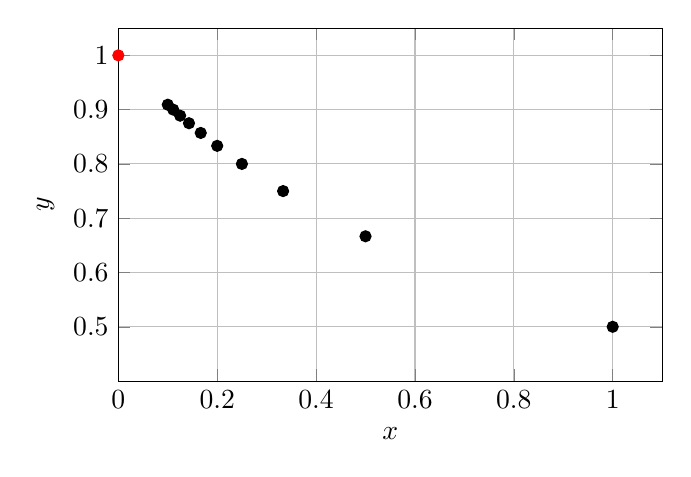
\begin{tikzpicture}
        \begin{axis}[
                xlabel={$x$},
                ylabel={$y$},
                xmin=0, xmax=1.1,
                ymin=0.4, ymax=1.05,
                xtick={0,0.2,0.4,0.6,0.8,1.0},
                ytick={0.5,0.6,0.7,0.8,0.9,1.0},
                grid=both,
                width=0.7\linewidth,
                height=0.5\linewidth
            ]
            % Punti della successione (approssimati in decimale)
            \addplot[only marks, mark=*] coordinates {
                (1.0,0.5)
                (0.5,0.6667)
                (0.3333,0.75)
                (0.25,0.8)
                (0.2,0.8333)
                (0.1667,0.8571)
                (0.1429,0.875)
                (0.125,0.8889)
                (0.1111,0.9)
                (0.1,0.9091)
            };
            % Evidenziamo il punto limite (0,1)
            \addplot[only marks, mark=*, red, mark size=2pt] coordinates {(0,1)};
            \node[red, below left] at (axis cs:0,1) {$(0,1)$};
        \end{axis}
    \end{tikzpicture}
    \end{center}
\end{exmp}

\vspace{10pt}

\paragraph{Punto interno}
\begin{bxthm}
\begin{defn}
    Siano $A\subseteq\mathbb{R}^n$ e $\overline{\mathbf{x}}\in A$. 
    Si dice che $\overline{\mathbf{x}}$ è \textbf{interno} ad $A$ se 
    \[\exists\,C\in\mathcal{C}_{\overline{\mathbf{x}}}\,:\;C\subseteq A.\]
\end{defn}
\end{bxthm}

\vspace{10pt}

I punti appartenenti al bordo del rettangolo non sono punti interni, poiché non esiste alcun cerchio con centro in un punto del bordo che sia interamente contenuto nel rettangolo. 
Al contrario, tutti i punti del rettangolo che non appartengono al bordo, sono punti interni, in quanto per ciascuno di essi è sempre possibile trovare un cerchio centrato nel punto stesso e 
completamente incluso nel rettangolo.
%fai disegno 

\vspace{10pt}

\begin{bxthm}
\begin{prop}
    Siano $A\subseteq\mathbb{R}^n$ e $\overline{\mathbf{x}}\in A$.
    Allora $\overline{\mathbf{x}}$ è interno ad $A$ se e solo se esiste un rettangolo di centro $\overline{\mathbf{x}}$ tale che $I\subseteq A$.
\end{prop}
\end{bxthm}
\begin{proof}\hfill
    \begin{itemize}
        \item[$\implies$]
        Per ipotesi, $\overline{\mathbf{x}}$ è interno ad $A$. Quindi 
        \[\exists\,C\in\mathcal{C}_{\overline{\mathbf{x}}}\,:\;C\subseteq A.\]
        Allora esiste un rettangolo $I$ di $\mathbb{R}^n$ di centro $\overline{\mathbf{x}}$ tale che $I\subseteq C$. 
        Poichè $C\subseteq A$, anche $I\subseteq A$.
        \item[$\impliedby$] 
        Per ipotesi, esiste un rettangolo $I$ di centro $\overline{\mathbf{x}}$ tale che $I\subseteq A$. 
        Allora \[\exists\,C\in\mathcal{C}_{\overline{\mathbf{x}}}\,:\;C\subseteq I.\]
        Poichè $I\subseteq A$, anche $C\subseteq A$. Allora $\overline{\mathbf{x}}$ è interno ad $A$.
    \end{itemize}
\end{proof}

\vspace{10pt}

\paragraph{Interno di un insieme}
\begin{bxthm}
\begin{defn}
    L'insieme dei punti interni ad $A$ si chiama \textbf{interno} di $A$ e si indica con $\dot{A}$ 
\end{defn}
\end{bxthm}

\vspace{10pt}

\paragraph{Insieme aperto}
\begin{bxthm}
\begin{defn}
    Diciamo che un insieme $A\subseteq\mathbb{R}^n$ è \textbf{aperto} se $A=\dot{A}$.
\end{defn}
\end{bxthm}

\vspace{10pt}

\begin{bxthm}
    \begin{prop}
    Un insieme $A\subseteq\mathbb{R}^n$ è aperto se e solo se ogni punto di $A$ è interno ad $A$.
    \end{prop}
\end{bxthm}
\begin{proof}\hfill
\begin{itemize}
    \item[$\implies$] Se $A$ è aperto, per definizione si ha $A=\dot{A}$; dunque ogni punto di $A$ è interno ad $A$.
    \item[$\impliedby$] Se ogni punto di $A$ è interno ad $A$, cioè $A\subseteq\dot{A}$, e poiché per definizione $\dot{A}\subseteq A$, ne consegue che $A=\dot{A}$. Perciò, $A$ è aperto.
\end{itemize}
\end{proof}

\vspace{10pt}

\begin{exmp}
    $A=\{(x,y)\in\mathbb{R}^2\,:\; x>0\land y>0\}$
    $\dot{A}=A$, $A$ è aperto perchè tutti i punti di $A$ sono interni ad $A$.
\end{exmp}

\vspace{10pt}

\paragraph{Punto di frontiera}
\begin{bxthm}
\begin{defn}
    Siano $A\subseteq\mathbb{R}^n$ e $\overline{\mathbf{x}}\in\mathbb{R}^n$.
    Allora si dice che $\overline{\mathbf{x}}$ è un punto di \textbf{frontiera} per $A$ se per ogni cerchio 
    di $\overline{\mathbf{x}}$, esistono sia punti di $A$ sia punti non appartenenti ad $A$.
    In simboli:
    \[
    \forall\, C\in\mathcal{C}_{\overline{\mathbf{x}}},\quad C\cap A\neq\emptyset \quad \land \quad C\cap (\mathbb{R}^n\setminus A)\neq\emptyset.
    \]
\end{defn}
\end{bxthm}

\vspace{10pt}

\begin{exmp}
    Tutti i punti sul bordo di un rettangolo sono di frontiera perchè in ogni cerchio di centro un punto del bordo ci sono sia punti del rettangolo sia punti non appartenenti al rettangolo.
\end{exmp}

\vspace{10pt}

\begin{exmp}
    Consideriamo l'insieme
    \[ A=\{(x,y)\in\mathbb{R}^2 : x>0 \ \text{e} \ y>0\}, \]
    allora i punti appartenenti al semiasse definito da \(x>0\) e quelli appartenenti al semiasse definito da \(y>0\) costituiscono punti di frontiera per \(A\). 
    Infatti, per ogni punto di tali semiasse, ogni cerchio (ossia, ogni cerchio centrato in quel punto) interseca sia l'insieme \(A\) sia il suo complementare.
\end{exmp}

\vspace{10pt}

\paragraph{Frontiera di un insieme}
\begin{bxthm}
\begin{defn}
    L'insieme dei punti di frontiera per $A$ è detto \textbf{frontiera} di $A$ e si indica con $\textup{Fr}(A)$ o $\partial A$.
\end{defn}
\end{bxthm}

\vspace{10pt}

% credo questo esempio sia sbagliato
%\begin{exmp}
%    Consideriamo un rettangolo definito come
%    \[
%    A = [a,b] \times [c,d] \subset \mathbb{R}^2.
%    \]
%    La frontiera di \( A \) è data dall'unione dei segmenti che costituiscono i lati del rettangolo.
%\end{exmp}

\vspace{10pt}

\begin{exmp}
    Per quanto riguarda un segmento chiuso \( A = [a,b] \subset \mathbb{R} \) (inteso come sottoinsieme dei reali), ogni punto del segmento risulta essere di frontiera, cioè
    \[
    \partial A = A.
    \]
\end{exmp}

\vspace{10pt}

\begin{exmp}
    Infine, considerando il primo quadrante
    \[
    A = \{(x,y) \in \mathbb{R}^2 : x>0 \text{ e } y>0\},
    \]
    la frontiera di \( A \) coincide con l'unione dei due semiasse positivi, formalmente espressa come
    \[
    \partial A = \{(x,0) : x > 0\} \cup \{(0,y) : y > 0\}.
    \]
\end{exmp}

\vspace{10pt}

\paragraph{Chiusura di un insieme}
\begin{bxthm}
\begin{defn}
    Si chiama \textbf{chiusura} di $A\subseteq\mathbb{R}^n$ l'insieme $\overline{A}=A\cup\partial A$. 
\end{defn}
\end{bxthm}

\vspace{10pt}

\paragraph{Insieme chiuso}
\begin{bxthm}
\begin{defn}
    Diciamo che un insieme $A\subseteq\mathbb{R}^n$ è \textbf{chiuso} se $A=\overline{A}$.
\end{defn}
\end{bxthm}

\vspace{10pt}

\begin{bxthm}
\begin{prop}
    Sia $A\subseteq\mathbb{R}^n$.
    Allora 
    \[A=\overline{A}\iff\forall\,x\in\overline{A},\;x\in A.\]
    o alternativamente
    \[A=\overline{A}\iff\overline{A}\subseteq A.\]
\end{prop}
\end{bxthm}
\begin{proof}
    Da
    \[\overline{A}=A\cup\partial A,\]
    segue che 
    \[A=\overline{A}\iff A=A\cup \partial A \iff\partial A\subseteq A.\]
\end{proof}

\vspace{10pt}

\begin{exmp}
Consideriamo i seguenti due insiemi in $\mathbb{R}^2$:
\begin{enumerate}
    \item Sia 
    \[
    A = [a,b] \times [c,d], \quad a,b,c,d\in\mathbb{R},\; a<b,\; c<d.
    \]
    Poiché per definizione l'intervallo chiuso $[a,b]$ contiene i suoi estremi, si ha
    \[
    \partial A \subset A,
    \]
    ovvero ogni punto di frontiera di $A$ appartiene ad $A$. Pertanto
    \[
    \overline{A} = A \quad \text{e } A \text{ è chiuso.}
    \]

    \item Sia
    \[
    B = \{(x,y)\in\mathbb{R}^2 : x>0 \text{ e } y>0\},
    \]
    che rappresenta il primo quadrante aperto. L'insieme dei punti di frontiera di $B$ è
    \[
    \partial B = \{(x,0) : x>0\}\cup\{(0,y) : y>0\}.
    \]
    Poichè nessun punto di $\partial B$ appartiene a $B$, si ha
    \[
    \partial B \not\subset B \quad \implies \quad \overline{B} = B\cup \partial B \neq B.
    \]
    Di conseguenza, l'insieme $B$ non è chiuso.
\end{enumerate}
\end{exmp}

\vspace{10pt}

Un altro concetto che ci serve è quello di punto di accumulazione e quello di punto isolato. 

\vspace{10pt}

\paragraph{Punto di accumulazione e punto isolato}
\begin{bxthm}
\begin{defn}
    Siano $A\subseteq\mathbb{R}^n$ e $\overline{\mathbf{x}}\in\mathbb{R}^n$. Diciamo che $\overline{\mathbf{x}}$ 
    è un \textbf{punto di accumulazione} per $A$ se \[\forall\,C\in\mathcal{C}_{\overline{\mathbf{x}}},\;A\cap C\setminus\{\overline{\mathbf{x}}\}\neq\emptyset.\]
    L'insieme dei punti di accumulazione si indica con \[\mathcal{D}(A)=\{\overline{\mathbf{x}}\in\mathbb{R}^n \ | \ \overline{\mathbf{x}} \textup{ è di accumulazione per }A\,\}.\]
    Se $\overline{\mathbf{x}}\in A$ non è di accumulazione per $A$, cioè se 
    \[\exists\,C\in\mathcal{C}_{\overline{\mathbf{x}}}\,:\;A\cap C=\{\overline{\mathbf{x}}\} \quad (\textup{o }A\cap C\setminus\{\overline{\mathbf{x}}\}=\emptyset), \]
    allora si dice che $\overline{\mathbf{x}}$ è \textbf{isolato}.
\end{defn}
\end{bxthm}

\vspace{10pt}

\begin{bxthm}
\begin{prop}
    Siano $A\subseteq\mathbb{R}^n$ e $\overline{\mathbf{x}}\in\mathbb{R}^n$.
    Allora $\overline{\mathbf{x}}\in\mathcal{D}(A)$ se e solo se $\forall\,C\in\mathcal{C}_{\overline{\mathbf{x}}}$, 
    esistono infiniti punti di $A$.
\end{prop}
\end{bxthm}

\vspace{10pt}

\begin{exmp}
    Consideriamo un cerchio nel piano. In esso, ogni punto del cerchio è un punto di accumulazione, sia che esso si trovi sul bordo sia che esso sia interno al cerchio. 
    Allo stesso modo, in un segmento ogni punto è di accumulazione. 
    Infine, nel caso del primo quadrante, i punti interni così come quelli appartenenti al bordo costituiscono punti di accumulazione.
\end{exmp}

\vspace{10pt}

\begin{bxthm}
\begin{prop}\hfill
    \begin{enumerate}
        \item $A\textup{ è chiuso}\iff\forall\,\mathbf{x}\in\mathcal{D}(A),\;\mathbf{x}\in A\;(\iff\mathcal{D}(A)\subseteq A)$;
        \item $\overline{\mathbf{x}}\in\partial A\,\cancel{\implies}\,\overline{\mathbf{x}}\in\mathcal{D}(A)$;
        \item $\overline{\mathbf{x}}\in\mathcal{D}(A)\,\cancel{\implies}\,\overline{\mathbf{x}}\in\partial A$.
    \end{enumerate}
\end{prop}
\end{bxthm}

\vspace{10pt}

\begin{rem}
Consideriamo due casi:
\begin{enumerate}
    \item \textbf{Il caso del rettangolo.}  
    Se $A$ è un rettangolo (cioè un prodotto di intervalli chiusi) in $\mathbb{R}^n$, ogni punto interno (cioè ogni punto che non appartiene al bordo) gode della proprietà che esiste un cerchio interamente contenuto in $A$.  
    In particolare, questo implica che:
    \begin{itemize}
        \item Ogni punto interno è un \textbf{punto di accumulazione} per $A$, poiché in ogni cerchio esso si trova insieme ad altri punti di $A$.
        \item Tuttavia, questi punti non sono punti di frontiera, perché non si ha l'intersezione dell'cerchio con $\mathbb{R}^n\setminus A$.
    \end{itemize}

    \item \textbf{Il caso degli isolati.}  
    Consideriamo l'insieme 
    \[
    A=\{(n,0)\,:\;n\in\mathbb{N}\}\subseteq\mathbb{R}^2.
    \]
    In questo insieme ogni punto $x_0=(n,0)$ è \textbf{isolato}, cioè esiste un cerchio $C\in\mathcal{C}_{(n,0)}$, con raggio sufficientemente piccolo da non includere né il punto precedente $(n-1,0)$ né il successivo $(n+1,0)$, tale che
    \[
    C\cap A=\{(n,0)\}.
    \]
    In questo caso:
    \begin{itemize}
        \item Poiché il punto è isolato, per definizione non può essere di accumulazione.
        \item Tuttavia, per ogni $n$, il punto $(n,0)$ appartiene comunque alla frontiera $\partial A$, poiché in ogni cerchio centrato in $(n,0)$ vi sono anche punti al di fuori di $A$. 
    \end{itemize}
\end{enumerate}

Questi esempi evidenziano alcune differenze chiave:
\begin{itemize}
    \item Un \textbf{punto interno} possiede intorni interamente contenuti in $A$ ed è automaticamente di accumulazione, ma non rientra nella frontiera.
    \item Un \textbf{punto di accumulazione} richiede che ogni cerchio contenga altri punti di $A$, mentre questo non implica che il punto sia di frontiera (dato che, se è interno, non si incontrano punti esterni).
    \item Un \textbf{punto isolato} è tale che esiste almeno un cerchio in cui non vi sono altri punti di $A$. Tali punti possono comunque appartenere alla frontiera, perché in ogni cerchio del punto si trovano anche punti di $\mathbb{R}^n\setminus A$, ma non sono di accumulazione.
\end{itemize}
\end{rem}

\vspace{10pt}

\begin{bxthm}
\begin{prop}
Sia $A\subseteq\mathbb{R}^n$. Allora $A$ è chiuso se e solo se per ogni successione $(x_k)_{k\in\mathbb{N}}$ tale che 
\[
    \forall\, k\in\mathbb{N},\;x_k\in A \quad \textup{ e } \quad \lim_{k\to+\infty} x_k = \mathbf{x},
\]
si ha che il limite $\mathbf{x}$ appartiene ad $A$. In altre parole, $A$ contiene tutti i limiti delle successioni di punti in $A$.
\end{prop}
\end{bxthm}

\vspace{10pt}

\paragraph{Insieme limitato}
\begin{bxthm}
\begin{defn}
    Si dice che $A\subseteq\mathbb{R}^n$ è \textbf{limitato} se $\exists$ un cerchio $C$ tale che $A\subseteq C$.    
\end{defn}
\end{bxthm}

\vspace{10pt}

\begin{bxthm}
\begin{prop}
    $A\subseteq\mathbb{R}^n$ è limitato se e solo se 
    \[\exists\, c>0 \,:\;\forall\,x\in A,\quad(\|x\|\leq c\;\textup{ e }\; \| x \|-\| \overline{\mathbf{x}} \|\leq \| x-\overline{\mathbf{x}} \|).\]
\end{prop}
\end{bxthm}
\begin{proof}\hfill 
    \begin{itemize}
        \item[$\implies$] Dalle ipotesi esiste un cerchio $C$ tale che $A\subseteq C$. 
        Sia $\overline{\mathbf{x}}$ il centro di $C$ e $r$ il suo raggio, avremo allora 
        \[C_{\overline{\mathbf{x}}}(r)=\{x\in\mathbb{R}^n\,:\;\| x-\overline{\mathbf{x}} \|<r\}.\]
        Poichè $A\subseteq C$, segue immediatamente che 
        \[\forall\, x\in A,\quad \| x-\overline{\mathbf{x}} \|<r.\]
        Dalla disuguaglianza triangolare 
        \[\| x \| -\| \overline{\mathbf{x}} \|\leq\| x-\overline{\mathbf{x}} \|<r \implies \| x \|-\| \overline{\mathbf{x}} \|<r \implies \| x \|<\| \overline{\mathbf{x}} \|+r.\]
        Ponendo $\| \overline{\mathbf{x}} \|+r=r$, ci troviamo con 
        \[\forall x\in A, \| x \| < c.\]

        \item[$\impliedby$] Dall'ipotesi si ha che esiste $c>0$ tale che
        \[
        \forall\, x\in A,\quad \|x\|\leq c.
        \]
        Consideriamo il cerchio chiuso centrato nell'origine di raggio $c$, definito da
        \[
        C_{0}(c)=\{x\in\mathbb{R}^n\,:\; \|x\|\leq c\}.
        \]
        Essendo che ogni elemento di $A$ ha norma minore o uguale a $c$, segue 
        \[
        A\subseteq C_{0}(c),
        \]
        cioè $A$ è limitato.
    \end{itemize}
\end{proof}

\vspace{10pt}

\begin{note}
    La prima parte della proposizione esprime la definizione classica di insieme limitato: esiste una costante $c>0$ tale che per ogni elemento $x\in A$ 
    la sua norma soddisfa $\|x\|\leq c$, cioè $A$ è contenuto in una palla centrata nell'origine di raggio $c$. La seconda disuguaglianza, 
    $\|x\|-\| \overline{\mathbf{x}} \|\leq \| x-\overline{\mathbf{x}} \|$, è una conseguenza della disuguaglianza triangolare (nella sua forma inversa) e indica che la 
    differenza tra la norma di $x$ e quella di un punto fisso $\overline{\mathbf{x}}$ è sempre minore o uguale alla distanza tra $x$ e $\overline{\mathbf{x}}$. 
    Questo fatto evidenzia come la "variazione" della norma, rispetto ad un punto fisso, sia controllata dalla distanza effettiva in $\mathbb{R}^n$. 
    Insieme, queste condizioni garantiscono che gli elementi di $A$ non "si allontanano" indefinitamente, cioè $A$ risulta limitato.
\end{note}

\vspace{10pt}

\paragraph{Insieme compatto}
\begin{bxthm}
\begin{defn}
    Si dice che $A\subseteq\mathbb{R}^n$ è \textbf{compatto} se è chiuso e limitato.
\end{defn}
\end{bxthm}

\vspace{10pt}

\paragraph{Insieme convesso}
\begin{bxthm}
\begin{defn}
    Si dice che $A\subseteq\mathbb{R}^n$ è \textbf{convesso} se 
    \[\forall\, \mathbf{x},\mathbf{y}\in A,\quad \overline{\mathbf{xy}}\subseteq A.\]
\end{defn}
\end{bxthm}

\vspace{10pt}

\paragraph{Insieme convesso per poligonali}
\begin{bxthm}
\begin{defn}
    Si dice che $A\subseteq\mathbb{R}^n$ è \textbf{convesso per poligonali} se per ogni coppia di punti 
    $\mathbf{x},\mathbf{y}$ di $A$ esiste una poligonale $P$ di estremi $\mathbf{x}$ e $\mathbf{y}$ tale che $P\subseteq A$.
\end{defn}
\end{bxthm}

\vspace{10pt}

\begin{note}
    Ogni insieme convesso possiede la proprietà che, per ogni coppia di punti al suo interno, il segmento che li unisce è contenuto in esso; pertanto, 
    essendo il segmento un caso particolare di poligonale, risulta che ogni insieme convesso è convesso per poligonale. 
    Tuttavia, la condizione inversa non è sempre verificata, come si nota nell'esempio della corona circolare, la quale ammette connessioni tramite 
    poligonali contenute nell'insieme pur non essendo convessa.
\end{note}

\vspace{10pt}

\paragraph{Insieme sconnesso}
\begin{bxthm}
\begin{defn}
    Si dice che $A\subseteq\mathbb{R}^n$ è \textbf{sconnesso} se esistono due insiemi aperti $A_1,A_2\subseteq\mathbb{R}^n$ tali che 
    \begin{enumerate}
        \item $A_1\cap A\neq\emptyset$ e $A_2\cap A\neq\emptyset$;
        \item $(A_1\cap A)\cap(A_2\cap A)=\emptyset$;
        \item $A=(A_1\cap A)\cup(A_2\cap A)$.
    \end{enumerate}
\end{defn}
\end{bxthm}

\vspace{10pt}

\paragraph{Insieme connesso}
\begin{bxthm}
\begin{defn}
    Si dice che $A\subseteq\mathbb{R}^n$ è \textbf{connesso} se non è sconnesso.
\end{defn}
\end{bxthm}

\vspace{10pt}

\begin{bxthm}
\begin{prop}
    Ogni insieme convesso per poligonale è anche connesso
\end{prop}
\end{bxthm}

\vspace{10pt}

\begin{bxthm}
\begin{prop}
   Sia $A\subseteq\mathbb{R}^n$ aperto.
   Allora $A$ è sconnesso se e solo se esistono due aperti $A_1$ e $A_2$ disgiunti e non vuoti tali che $A=A_1\cup A_2$.
\end{prop}
\end{bxthm}

\vspace{10pt}

\begin{bxthm}
\begin{thm}
    Sia $A\subseteq\mathbb{R}^n$ aperto.
    Allora $A$ è connesso se e solo se è convesso per poligonale.
\end{thm}
\end{bxthm}

\vspace{10pt}

Alla luce di quanto esposto, definiamo una funzione reale di due variabili come un'applicazione
\[
f: A \subseteq \mathbb{R}^2 \to \mathbb{R},\quad (x, y) \mapsto f(x, y).
\]
Analogamente, una funzione di tre variabili è data da
\[
f: A \subseteq \mathbb{R}^3 \to \mathbb{R},\quad (x, y, z) \mapsto f(x, y, z),
\]
mentre nel caso generale di una funzione di $n$ variabili si scrive
\[
f: A \subseteq \mathbb{R}^n \to \mathbb{R},\quad \mathbf{x} = (x_1, x_2, \dots, x_n) \mapsto f(x_1, x_2, \dots, x_n) = f(\mathbf{x}).
\]

\vspace{10pt}

% Esempi e osservazioni sulle funzioni e sui relativi grafici

% Esempio 1: Funzione in due variabili con dominio definito da un'inequazione lineare
Sia ad esempio 
\[
f(x,y)=\sqrt{\,y-x\,}.
\]
Per garantire il significato dell'espressione (cioè, che la radice quadrata sia definita nel campo dei numeri reali) è necessario richiedere
\[
y-x\ge 0 \quad\implies\quad y\ge x.
\]
Pertanto la funzione 
\[
f \colon A \subseteq \mathbb{R}^2 \to \mathbb{R}, \qquad f(x,y)=\sqrt{y-x},
\]
è definita sull'insieme
\[
A=\{(x,y)\in\mathbb{R}^2 \;:\; y\ge x\}\,.
\]

% Esempio 2: Funzione in due variabili con dominio definito da un'inequazione quadratica (relativa a una palla)
Sia invece 
\[
f(x,y)=\frac{1}{\sqrt{x^2+y^2-1}}\,.
\]
L'espressione sotto radice deve essere strettamente positiva; notiamo che
\[
x^2+y^2-1>0 \quad\implies\quad x^2+y^2>1\,.
\]
Quindi, la funzione è definita in
\[
A=\{(x,y)\in\mathbb{R}^2 \;:\; x^2+y^2>1\}\,,
\]
escludendo la frontiera del cerchio (ossia il luogo in cui \(x^2+y^2=1\)).


\paragraph{Grafico di una funzione di una variabile: funzione reale di una sola variabile}
% (il grafico risiede in R^2)
Sia \(f : I \subseteq \mathbb{R} \to \mathbb{R}\) una funzione di una sola variabile. Il grafico di \(f\) è definito dall'insieme
\[
G_f=\{(x,y)\in\mathbb{R}^2 \;:\; x\in I \text{ e } y=f(x)\}\,.
\]


\paragraph{Grafico di una funzione di due variabili: funzione reale di due variabili, grafico in $\mathbb{R}^3$}
Sia ora \(f : A \subseteq \mathbb{R}^2 \to \mathbb{R}\) una funzione di due variabili. Il relativo grafico è 
\[
G_f=\{(x,y,z)\in\mathbb{R}^3 \;:\; (x,y)\in A \text{ e } z=f(x,y)\}\,.
\]


\paragraph{Grafico in dimensione maggiore: funzione di $n$ variabili}
Generalmente, per una funzione \(f : A \subseteq \mathbb{R}^n \to \mathbb{R}\) (con
\[
f(x_1,x_2,\dots,x_n)=f(x)),
\]
il grafico di \(f\) è definito come
\[
G_f=\{(x_1,x_2,\dots,x_n,z)\in\mathbb{R}^{n+1} \;:\; x=(x_1,\dots,x_n)\in A \text{ e } z=f(x)\}\,.
\]
In particolare, quando \(f\colon \mathbb{R}^3\to\mathbb{R}\), il grafico \(G_f\) si considera un sottoinsieme di \(\mathbb{R}^4\).

\paragraph{Definizione formale di limite per una funzione di una variabile}
Sia \(f : I \subseteq \mathbb{R} \to \mathbb{R}\) una funzione e sia \(x_0\) un punto di accumulazione di \(I\). 
Si dice che 
\[
\lim_{x\to x_0}f(x)=l\in\mathbb{R}
\]
se
\[
\forall\,\varepsilon>0,\ \exists\,\delta>0 \text{ tale che } \forall\, x\in I \text{ con } 0<|x-x_0|<\delta,\quad |f(x)-l|<\varepsilon\,.
\]
In altre parole, per ogni cerchio di \(l\) (cioè, per ogni intervallo aperto centrato in \(l\) di ampiezza \(\varepsilon\)), si può trovare un cerchio di \(x_0\) (cioè un intervallo aperto centrato in \(x_0\) di raggio \(\delta\)) tale che ogni \(x\neq x_0\) in tale cerchio soddisfi \(f(x)\in (l-\varepsilon,l+\varepsilon)\).

Un'alternativa sintetica per esprimere la definizione è:
\[
\lim_{x\to x_0} f(x)=l \quad \iff \quad x\sim x_0,\;\implies f(x)\sim l\,.
\]
Questa espressione evidenzia il fatto che, avvicinandosi a \(x_0\), i valori di \(f\) si avvicinano ad \(l\).

\vspace{10pt}

\paragraph{Limite per una funzione a $n$ variabili}
\begin{bxthm}
\begin{defn}
    Siano $f:A\subseteq\mathbb{R}^n\to\mathbb{R}$ e $\overline{\mathbf{x}}\in\mathcal{D}(A)$. 
    Si dice che 
    \[\lim_{\mathbf{x}\to \overline{\mathbf{x}}}=l\in\mathbb{R}\]
    se 
    \[\forall\, \varepsilon>0\,,\; \exists\, \delta>0\,:\;\forall\, \mathbf{x}\in A,\quad 0<\| \mathbf{x}-\overline{\mathbf{x}} \|<\delta\implies | f(\mathbf{x})-l |<\varepsilon.\]
\end{defn}
\end{bxthm}

\vspace{10pt}

% Definizioni riguardanti il limite di una funzione

% La condizione 0 < \|x - x₀\| < δ significa che:
\[
0 < \|\mathbf{x}-\overline{\mathbf{x}}\| < \delta \quad \iff \quad \mathbf{x} \in C_{\overline{\mathbf{x}}}(\delta) \setminus \{\overline{\mathbf{x}}\},
\]
dove \(C_{\overline{\mathbf{x}}}(\delta)\) è un cerchio di centro \(\overline{\mathbf{x}}\) e raggio \(\delta\).

% Definizione del limite finito
Definiamo il limite di \(f\) in \(x_0\) nel seguente modo:
\[
\lim_{x\to x_0} f(x) = l \in \mathbb{R} \quad \iff \quad \forall\, J\in\mathcal{I}_l,\; \exists\, \delta > 0\,:\; \forall\, x \in A,\quad 0 < \|x - x_0\| < \delta\implies f(x) \in J.
\]
In altre parole, se \(x\) si avvicina a \(x_0\) (ovvero \(x \sim x_0\)), allora \(f(x)\) si avvicina a \(l\) (cioè \(f(x) \sim l\)).

% Definizione del limite infinito (positivo)
Si dice che
\[
\lim_{x\to x_0} f(x) = +\infty \quad \iff \quad \forall\, M > 0,\; \exists\, \delta > 0\,:\;\forall\, x \in A,\; 0 < \|x - x_0\| < \delta\implies f(x) > M.
\]

% Definizione del limite infinito (negativo)
Analogamente, si dice che
\[
\lim_{x\to x_0} f(x) = -\infty \quad \iff \quad \forall\, M < 0,\; \exists\, \delta > 0 \,:\; \forall\, x \in A,\; 0 < \|x - x_0\| < \delta\implies f(x) < M.
\]

\vspace{10pt}

\paragraph{Funzione continua in un punto}
\begin{bxthm}
\begin{defn}
    Sia $f:A\subseteq\mathbb{R}^n\to\mathbb{R}$ e sia $\overline{\mathbf{x}}\in A$. 
    Si dice che $f$ è \textbf{continua} in $\overline{\mathbf{x}}$ se 
    \[\forall\,\varepsilon>0,\;\exists\,\delta>0\,:\;\forall\, \mathbf{x}\in A,\quad\| \mathbf{x}-\overline{\mathbf{x}} \|<\delta \implies|f(\mathbf{x})-f(\overline{\mathbf{x}})|<\varepsilon.\]
    Alternativamente, 
    \[\forall\,\varepsilon>0,\;\exists\,C\in\mathcal{C}_{\overline{\mathbf{x}}}\,:\;\forall\, \mathbf{x}\in A\cap C,\quad|f(\mathbf{x})-f(\overline{\mathbf{x}})|<\varepsilon.\]
\end{defn}
\end{bxthm}

\vspace{10pt}

\begin{note}
$f$ è continua in $\overline{\mathbf{x}} \iff \forall\varepsilon>0,\;\exists\,C\in\mathcal{C}_{\overline{\mathbf{x}}}\,:\; 
\forall\, \mathbf{x}\in A\cap C, |f(\mathbf{x})-f(\overline{\mathbf{x}})|<\varepsilon.$
Se $\mathbf{x}\sim \overline{\mathbf{x}}$, $f(\mathbf{x})\sim f(\overline{\mathbf{x}})$
\end{note}

\vspace{10pt}

\begin{bxthm}
\begin{prop}\hfill
\begin{enumerate}
    \item Se $\overline{\mathbf{x}}$ è un punto isolato per $A$, ogni funzione è continua in $\overline{\mathbf{x}}$;
    \item Se $\overline{\mathbf{x}}\in\mathcal{D}(A)$, $f$ è continua in $\overline{\mathbf{x}} \iff \lim\limits_{\mathbf{x}\to \overline{\mathbf{x}}}f(\mathbf{x})=f(\overline{\mathbf{x}})$.
\end{enumerate}
\end{prop}
\end{bxthm}
\begin{proof}\hfill 
    \begin{enumerate}
        \item Sia $\overline{\mathbf{x}}$ un punto isolato. Allora 
        \[\exists\,\overline{C}\in\mathcal{C}_{\overline{\mathbf{x}}}\,:\;\overline{C}\cap A=\{\overline{\mathbf{x}}\}.\]
        Siano $\varepsilon>0$ e  $C=\overline{C}$. Poichè $C\cap A=\{\overline{\mathbf{x}}\}$, avremo che $|f(\overline{\mathbf{x}})-f(\overline{\mathbf{x}})|=0<\varepsilon$.
        \item Sia $\overline{\mathbf{x}}$ di accumulazione per $A$. Allora 
        \[\lim_{\mathbf{x}\to \overline{\mathbf{x}}} f(\mathbf{x})=f(\overline{\mathbf{x}})\iff \forall\,\varepsilon>0,\;\exists\,\delta>0\,:\; \forall\, \mathbf{x}\in A,\quad 0<\|\mathbf{x}-\overline{\mathbf{x}}\|<\delta\implies |f(\mathbf{x})-f(\overline{\mathbf{x}})|<\varepsilon.\] 
        La condizione $|f(\mathbf{x})-f(\overline{\mathbf{x}})|<\varepsilon$ vale $\forall\, \mathbf{x}\in A$ con $\| \mathbf{x}-\overline{\mathbf{x}} \|<\delta$, cioè $f$ è continua in $\overline{\mathbf{x}}$.
    \end{enumerate}
\end{proof}

\vspace{10pt}

\paragraph{Funzione continua}
\begin{bxthm}
\begin{defn}
    Si dice che $f$ è continua in $A$ se è continua in ogni punto di $A$.
    In simboli,
    \[\forall\, \overline{\mathbf{x}}\in A,\;\forall\,\varepsilon>0,\;\exists\,\delta>0\,:\;\forall\, \mathbf{x}\in A,\quad\| \mathbf{x}-\overline{\mathbf{x}} \|<\delta \implies|f(\mathbf{x})-f(\overline{\mathbf{x}})|<\varepsilon.\]
\end{defn}
\end{bxthm}

\vspace{10pt}

\paragraph{Funzione uniformemente continua}
\begin{bxthm}
\begin{defn}
    Si dice che $f$ è uniformemente continua in $A$ se 
    \[\forall\,\varepsilon>0,\;\exists\,\delta>0\,:\;\forall\, x,y\in A,\quad\| x-y \|<\delta\implies |f(x)-f(y)|<\varepsilon.\]
\end{defn}
\end{bxthm}

\vspace{10pt}

\begin{note}
    Questa definizione è più forte della normale continuità poichè la implica, mentre non è vero il contrario.
\end{note}

\vspace{10pt}

\paragraph{Teorema di Cantor}
\begin{bxthm}
\begin{thm}
    Sia $f:A\subseteq\mathbb{R}^n\to\mathbb{R}$ continua con $A$ compatto.
    Allora $f$ è uniformemente continua.
\end{thm}
\end{bxthm}

\vspace{10pt}

\paragraph{Teorema di Weierstrass}
\begin{bxthm}
\begin{thm}
    Sia $f:A\subseteq\mathbb{R}^n\to\mathbb{R}$ continua con $A$ compatto.
    Allora $f$ ha minimo e massimo. In simboli 
    \[\exists\,x_1,x_2\in A\,:\;\forall\, x\in A,\;f(x_1)\leq f(x)\leq f(x_2).\]
\end{thm}
\end{bxthm}

\vspace{10pt}

\paragraph{Teorema della permanenza del segno}
\begin{bxthm}
\begin{thm}
    Sia $f:A\subseteq\mathbb{R}^n\to\mathbb{R}$ continua con $f(\overline{\mathbf{x}})>0$. Allora 
    \[\exists\,C\in\mathcal{C}_{\overline{\mathbf{x}}}\,:\;\forall x\in A\cap C,\; f(x)>0.\]
\end{thm}
\end{bxthm}

\vspace{10pt}

\paragraph{Teorema dei valori intermedi}
\begin{bxthm}
\begin{thm}
    Sia $f:A\subseteq\mathbb{R}^n\to\mathbb{R}$ continua con $A$ limitato e connesso.
    Allora $f$ assume tutti i valori compresi tra l'estremo inferiore e l'estremo superiore.
    Cioè ponendo $m=\inf\{f(x):x\in A\}$ e $M=\sup\{f(x):x\in A\}$, avremo che 
    \[\forall\,\alpha\in\,]m,M[\,,\;\exists\,\overline{\mathbf{x}}\in A\,:\;f(\overline{\mathbf{x}})=\alpha.\]
\end{thm}
\end{bxthm}

\vspace{10pt}

\section{Coordinate polari}

\vspace{10pt}
Fissiamo un'unità di misura per le lunghezze, una per gli angoli, e un verso di percorrenza per gli angoli.
Sia $P$ un punto nel piano diverso dal polo $P_0$.
Allora si definisce \textbf{modulo} $\rho$ di $P$ la lunghezza del segmento $\overline{P_0P}$, e 
\textbf{anomalia} $\theta$ di $P$ la misura dell'angolo che la semiretta $r$ forma con la semiretta $\overline{P_0P}$.
Chiamiamo $\rho$ e $\theta$ \textbf{coordinate polari} di $P$.
Se $P=P_0$, allora diciamo che il modulo è uguale a zero e l'anomalia non è definita.
$\rho$ ci dice che $P$ si trova nella circonferenza di centro $P_0$ e raggio $\rho$.

\paragraph{Passaggio da coordinate cartesiane a polari e viceversa}
Ci sono delle formule che permettono di passare dalle coordinate polari a quelle cartesiane e viceversa. 
Per ottenre queste formule prendiamo un riferimento cartesiano in cui la semiretta $r$ coincide con il semiasse $x$ positivo e quindi il polo $P_0$ coinciderà con l'origine delle coordinate.

Poichè $\rho$ è la lunghezza del segmento $\overline{P_0P}$, $\rho$ coincide con la distanza di $P$ da $(0,0)$. 
Se denotiamo con $x$ e $y$ le coordinate cartesiane del punto $P$, 
la distanza di $P$ dall'origine è $\rho=\sqrt{x^2+y^2}$.
Per le formule trigonometriche, abbiamo
\begin{equation}
    \begin{cases}
        x=\rho\cos \vartheta\\
        y=\rho\sin \vartheta
    \end{cases}\label{coord}  
\end{equation}
Se conosciamo $\rho$ e $\vartheta$, ci ricaviamo $x$ e $y$ da \ref{coord}. 
Viceversa, se conosciamo $x$ e $y$, seguirà $\rho=\sqrt{x^2+y^2}$ e da \ref{coord} 
\[\cos v=\dfrac{x}{\rho}\quad \sin x=\dfrac{y}{\rho}.\]

\vspace{10pt}

\begin{exmp}
    Sia $P=(1,1)$. Allora $\rho=\sqrt{1^2+1^2}=\sqrt{2}$. Da cui 
    \[\begin{cases}
        x=\rho\cos\vartheta\\
        y=\rho\sin\vartheta
    \end{cases}=\begin{cases}
        1=\sqrt{2}\cos\vartheta\\
        1=\sqrt{2}\sin\vartheta
    \end{cases}\implies \cos\vartheta=\dfrac{\sqrt{2}}{2}=\sin\vartheta\implies \vartheta=\dfrac{\pi}{4}.\]
    Sia $P=(2,\frac{\pi}{3})$.
\end{exmp}

\vspace{10pt}

\paragraph{Caso in cui $P_0\neq(0,0)$}
Prendiamo un riferimento cartesiano in cui la semiretta $r$ sia parallela al semiasse $x$ positivo, e $P_0=(x_0,y_0)\neq(0,0)$.
Dato un $P(x,y)\neq P_0$, avremo che $\rho=\sqrt{(x-x_0)^2+(y-y_0)^2}$, dunque 
\[\begin{cases}
        x-x_0=\rho\cos\vartheta\\
        y-y_0=\rho\sin\vartheta
    \end{cases}=\begin{cases}
        x=\rho\cos\vartheta+x_0\\
        y=\rho\sin\vartheta+y_0
    \end{cases}.\]

\vspace{10pt}

Ogni volta che si assegna un valore a una variabile in una funzione a due variabili, si ottiene una funzione che dipende solo dall'altra variabile (l'altra è diventata un parametro) rispetto a un punto fisso.
Ad esempio, data $f(x,y)=\sqrt{x^2+y^2}$, troviamo che per $y=1$, abbiamo $f(x)={x^2+1}$.
Questo ci permette di introdurre le funzioni parziali.

\vspace{10pt}

\paragraph{Funzioni parziali}
\begin{bxthm}
\begin{defn}\label{funzparz}
    Siano $f:A\subseteq\mathbb{R}^2\to\mathbb{R}$ e $(x_0,y_0)\in\mathbb{R}^2$.
    Definiamo le seguenti \[\varphi :x\to f(x,y_0)\quad\psi :y\to f(x_0,y).\]
    $\varphi$ e $\psi$ si chiamano \textbf{funzioni parziali} generate da $f$ rispetto a $(x_0,y_0)$.
    Geometricamente, $\varphi\;(\psi)$  può essere vista come $f$ calcolata lungo la retta $y=y_0\;(x=x_0)$.
    %Aggiungere quì disegno sulle note
    Non è detto che $\varphi$ e $\psi$ siano ben definiti.
    $\varphi$ è definita in \[A_\varphi=\{x\,|\,(x,y_0)\in A\},\] mentre $\psi$ è definita in \[A_\psi=\{y\,|\,(x_0,y)\in A\}.\]
    Inoltre, 
    \[(x_0,y_0)\in A\implies x_0\in A_\varphi\;\land\;y_0\in A_\psi.\]
\end{defn}
\end{bxthm}

\vspace{10pt}

\begin{bxthm}
\begin{thm}
    Se $(x_0,y_0)$ è interno ad $A$, allora $x_0$ è interno ad $A_\varphi$ e $y_0$ è interno ad $A_\psi$.
    In simboli:
    \[(x_0,y_0)\in\dot{A}\implies\exists\, r>0\,:\;[x_0-r,x_0+r]\subseteq A_\varphi\;\land\;[y_0-r,y_0+r]\subseteq A_\psi.\]
\end{thm}
\end{bxthm}
\begin{proof}
    Poichè $(x_0,y_0)\in\dot{A}$, $\exists$ un cerchio $C$ di centro $(x_0,y_0)$ tale che $C\subseteq A$. Sia $r$ il raggio di $C$.
    Dimostriamo che $[x_0-r,x_0+r]\subseteq A_\varphi$. 
    Da $x\in [x_0-r,x_0+r]$ abbiamo $|x-x_0|\leq r$.
    Dimostriamo che $(x,y_0)\in C$.
    \[\| (x,y_0)-(x_0,y_0) \|=\| (x-x_0,0) \|=\sqrt{(x-x_0)^2}=|x-x_0|\leq r\implies (x,y_0)\in C.\]
    Poichè $C\subseteq A$, avremo che $(x,y_0)\in A$ da cui $x\in A_\varphi$.
    In maniera analoga si dimostra che $[y_0-r,y_0+r]\subseteq A_\psi$.
\end{proof}

\vspace{10pt}

\begin{note}
    Se $(x_0,y_0)\in \partial A$, $\varphi$ e $\psi$ potrebbero essere definite solo in un punto.
    Siano ad esempio
    \[A=C_{(0,0)}(1),\quad (x_0,y_0)=(0,1),\quad \varphi(x)=f(x,1).\]
    I punti $(x,1)$ sono i punti della retta $y=1$, che incontra $A$ solo nel punto $(0,1)$.
    %fare disegno
\end{note}

\vspace{10pt}

\paragraph{Teorema sui limiti delle funzioni parziali}
\begin{bxthm}
\begin{thm}
    Siano $f:A\subseteq\mathbb{R}^2\to\mathbb{R}$ e $(x_0,y_0)\in\mathcal{D}(A)$.
    Supponiamo che 
    \[\lim_{(x,y)\to(x_0,y_0)}f(x,y)=l\in\overline{\mathbb{R}}.\]
    Allora 
    \[x_0\in\mathcal{D}(A_\varphi)\implies \lim_{x\to x_0}\varphi(x)=l\quad\land\quad y_0\in\mathcal{D}(A_\psi)\implies \lim_{y\to y_0}\psi(y)=l.\]
\end{thm}
\end{bxthm}
\begin{proof}
    Sia $l\in\mathbb{R}$, per $\pm\infty$ la dimostrazione è analoga. 
    Sia $x_0\in\mathcal{D}(A_\varphi)$. Vogliamo dimostrare che $\lim\limits_{x\to x_0}\varphi(x)=l$,
    cioè che
    \[\forall\,\varepsilon>0,\;\exists\,\delta>0\,:\;\forall\, x\in A_\varphi,\quad 0<|x-x_0|<\delta\implies|\varphi(x)-l|<\varepsilon.\]
    Per ipotesi, 
    \[\forall\,\varepsilon>0,\;\exists\,\delta>0\,:\;\forall\,(x,y)\in A,\quad 0<\|(x,y)-(x_0,y_0)\|<\delta\implies|f(x,y)-l|<\varepsilon.\]
    Prendiamo $\varepsilon>0$ e $\delta$ come nell'ipotesi. 
    Sia $x\in A_\varphi$ con $0<|x-x_0|<\delta$ e ricordiamo che $x\in A_\varphi\implies(x,y_0)\in A$.
    Abbiamo dunque 
    \[\| (x,y_0)-(x_0,y_0) \|=\|(x-x_0)\|=\sqrt{(x-x_0)^2}=|x-x_0|\implies 0<\|(x,y)-(x_0,y_0)\|<\delta.\]
    In conclusione,
    \[((x,y_0)\in A \;\land\; 0<\| (x,y)-(x_0,y_0) \|<\delta)\implies |f(x,y_0)-l|<\varepsilon\implies |\varphi(x)-l|<\varepsilon\implies f(x,y_0)=\varphi(x).\]
\end{proof}

\vspace{10pt}

Il teorema dice che se $f$ ha un limite $l$ in un punto $(x_0,y_0)$, $f$ ha lo stesso limite lungo la retta $y=y_0$ e lungo la retta $x=x_0$.
Segue ovviamente che 
\[\lim_{x\to x_0}\varphi(x)\neq\lim_{y\to y_0}\psi(y)\implies\nexists\lim_{(x,y)\to(x_0,y_0)}f(x,y).\]

\vspace{10pt}

\begin{exmp}
    Sia ad esempio la seguente funzione 
    \[f:A=\mathbb{R}^2\setminus\{(0,0)\}\to\mathbb{R},\quad (x,y)\mapsto\dfrac{x^2}{x^2+y^2}.\]
    \begin{center}
        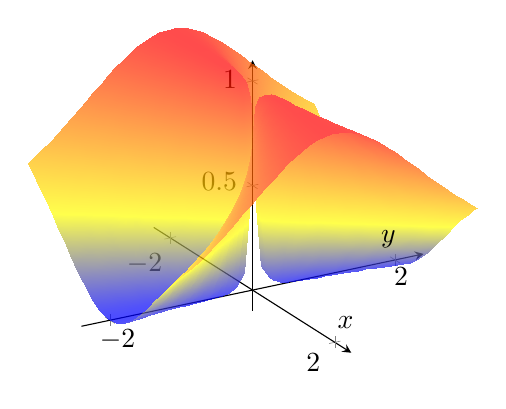
\begin{tikzpicture}
            \begin{axis}[
                view={60}{30}, % Angolazione della vista
                axis lines=center,
                xlabel={$x$},
                ylabel={$y$},
                domain=-2:2,
                y domain=-2:2,
                samples=40,
                samples y=40,
                enlargelimits=true,
                colormap/hot
            ]
                \addplot3[
                    surf,
                    shader=interp,
                    opacity=0.7,
                ]
                {x^2/(x^2 + y^2)};
            \end{axis}
        \end{tikzpicture}
        \hspace{1cm}
        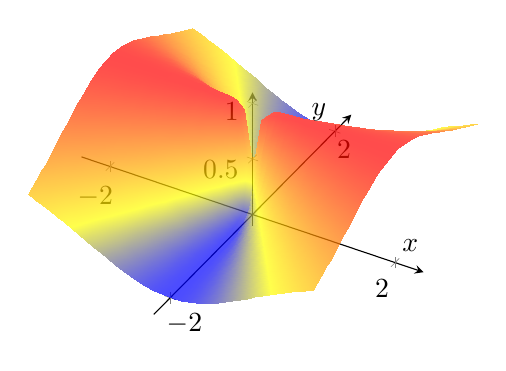
\begin{tikzpicture}
            \begin{axis}[
                view={30}{60}, % Angolazione della vista
                axis lines=center,
                xlabel={$x$},
                ylabel={$y$},
                domain=-2:2,
                y domain=-2:2,
                samples=40,
                samples y=40,
                enlargelimits=true,
                colormap/hot
            ]
                \addplot3[
                    surf,
                    shader=interp,
                    opacity=0.7,
                ]
                {x^2/(x^2 + y^2)};
            \end{axis}
        \end{tikzpicture}
    \end{center}
    Abbiamo che $(0,0)\in\mathcal{D}(A)$.
    Calcoliamo i limiti delle funzioni parziali nell'origine: 
    \[\varphi(x)=f(x,0)=\dfrac{x^2}{x^2+0}=\dfrac{x^2}{x^2}=1,\quad\psi(y)=f(0,y)=\dfrac{0}{0+y^2}=0,\]
    i due limiti differiscono, dunque possiamo concludere che $\nexists\lim_{(x,y)\to(0,0)}f(x,y)$.
\end{exmp}

\vspace{10pt}

Non vale però il viceversa del teorema, cioè se $\lim\limits_{x\to x_0}\varphi(x)=\lim\limits_{y\to y_0}\psi(y)$, non possiamo concludere che $\exists\lim_{(x,y)\to(x_0,y_0)}f(x,y)$.

\vspace{10pt}

\begin{exmp} 
    Sia ad esempio la seguente funzione 
    \[f:A=\mathbb{R}^2\setminus\{(0,0)\}\to\mathbb{R},\quad (x,y)\mapsto\dfrac{xy}{x^2+y^2}.\]
    \begin{center}
        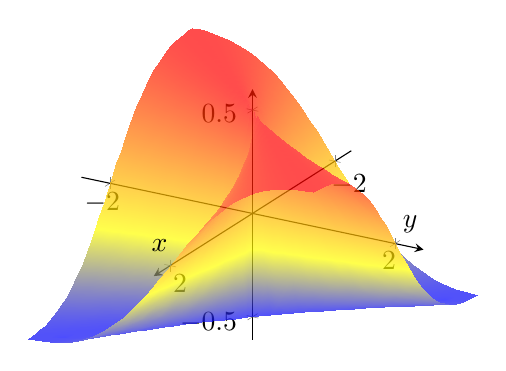
\begin{tikzpicture}
            \begin{axis}[
                view={120}{30}, % Angolazione della vista
                axis lines=center,
                xlabel={$x$},
                ylabel={$y$},
                domain=-2:2,
                y domain=-2:2,
                samples=40,
                samples y=40,
                enlargelimits=true,
                colormap/hot
            ]
                \addplot3[
                    surf,
                    shader=interp,
                    opacity=0.7,
                ]
                {x*y/(x^2 + y^2)};
            \end{axis}
        \end{tikzpicture}
        \hspace{1cm}
        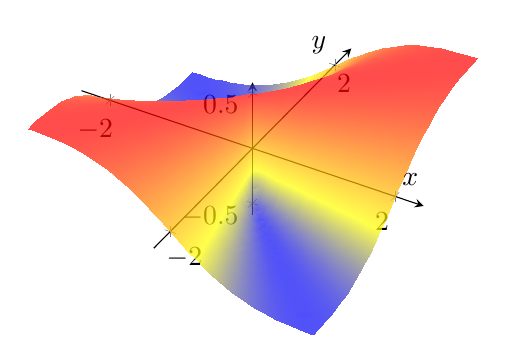
\begin{tikzpicture}
            \begin{axis}[
                view={30}{60}, % Angolazione della vista
                axis lines=center,
                xlabel={$x$},
                ylabel={$y$},
                domain=-2:2,
                y domain=-2:2,
                samples=40,
                samples y=40,
                enlargelimits=true,
                colormap/hot
            ]
                \addplot3[
                    surf,
                    shader=interp,
                    opacity=0.7,
                ]
                {x*y/(x^2 + y^2)};
            \end{axis}
        \end{tikzpicture}
    \end{center}
    Calcoliamo i limiti delle funzioni parziali nell'origine: 
    \[\varphi(x)=f(x,0)=\dfrac{x\cdot0}{x^2+0}=0,\quad\psi(y)=f(0,y)=\dfrac{0\cdot y}{0+y^2}=0,\]
    $\varphi$ e $\psi$ sono definite in $\mathbb{R}\setminus\{0\}$ e hanno limite $0$ in $0$, dunque secondo il teorema precedente dovremo avere $\lim_{(x,y)\to(0,0)}\dfrac{xy}{x^2+y^2}=0$, ma non è così perchè il limite non esiste.
    Dire che 
    \[\lim_{(x,y)\to(0,0)}\dfrac{xy}{x^2+y^2}=0\]
    equivale a dire che 
    \[\forall\,\varepsilon>0,\;\exists\,C\in\mathcal{C}_{(0,0)}\,:\;\forall\,(x,y)\in C\cap A\setminus\{(0,0)\},\quad\left|\dfrac{xy}{x^2+y^2}\right|<\varepsilon.\]
    Per dimostrare che 
    \[\lim_{(x,y)\to(0,0)}\dfrac{xy}{x^2+y^2}\neq0,\]
    dobbiamo negare la proposizione sudetta, ossia dimostrare che
    \[\exists\,\varepsilon>0\,:\;\forall\, C\in\mathcal{C}_{(0,0)},\; \exists\,(x,y)\in C\cap A\setminus\{(0,0)\}\,:\;\left|\dfrac{xy}{x^2+y^2}\right|\geq\varepsilon.\]
    Sulla bisettrice $y=x$, $f$ diventa $\dfrac{x^2}{x^2+x^2}=\dfrac{1}{2}$. In ogni cerchio di centro $(0,0)$, esistono punti della bisettrice in cui $f=\frac{1}{2}$.
    Sia $0<\varepsilon\leq\dfrac{1}{2}$. Se $C$ è un cerchio di centro $(0,0)$, in $C$ $\exists$ punti in cui $f=\dfrac{1}{2}\geq\varepsilon$
    \[\implies\lim_{(x,y)\to(0,0)}\neq0\implies\nexists\lim_{(x,y)\to(0,0)}\dfrac{xy}{x^2+y^2}.\]
\end{exmp}

\vspace{10pt}

\begin{bxthm}
\begin{cor}
Se $f:A\subseteq\mathbb{R}^2\to\mathbb{R}$ è continua in un punto $(x_0,y_0)\in A$, $\varphi$ è continua in $x_0$ e $\psi$ è continua in $y_0$.
Se $\varphi$ è continua in $x_0$ e $\psi$ è continua in $y_0$, si dice che $f$ è \textbf{separatamente continua} in $(x_0,y_0)$.
\end{cor}
\end{bxthm}
\begin{proof}
    Come primo passo, dimostriamo che se $(x_0,y_0)$ è isolato per $A$, allora $x_0$ è isolato per $A_\varphi$ e $y_0$ è isolato per $A_\psi$.
    Se $(x_0,y_0)$ è isolato per $A$, allora $\exists\,C\in\mathcal{C}_{(x_0,y_0)}\,:\;C\cap A=\{(x_0,y_0)\}$.
    Sia dunque $r$ il raggio di $C$.
    Dal teorema abbiamo che 
    \[[x_0-r,x_0+r]\cap A_\varphi=\{x_0\}\quad\land\quad[y_0-r,y_0+r]\cap A_\psi=\{y_0\},\]
    da cui possiamo estrarre
    \[\{x_0\}\subseteq[x_0-r,x_0+r]\cap A_\varphi.\]
    Sia ora $x\in[x_0-r,x_0+r]\cap A_\varphi$, da \ref{funzparz} sappiamo che $x\in A_\varphi\implies(x,y_0)\in A$.
    Poichè $x\in[x_0-r,x_0+r]$, avremo che $\| (x,y_0)-(x_0,y_0) \|=\|(x-x_0,0)\|=|x-x_0|\leq r$.
    Dunque $(x,y_0)\in C\implies x=x_0$.
    %\[\| (x,y_0)-(x_0,y_0) \|=|x-x_0|\leq r\implies (x,y_0)\in C. (x,y_0)\in C\cap A=\{(x_0,y_0)\}\implies x=x_0.\]
\end{proof}

\vspace{10pt}

\begin{note}
    Dunque se $f$ è continua in $(x_0,y_0)$, allora è anche separatamente continua in $(x_0,y_0)$, mentre il viceversa non vale.
\end{note}

\vspace{10pt}

\begin{exmp}
Sia ad esempio 
\[f:A\subseteq\mathbb{R}^2\to\mathbb{R},\quad (x,y)\mapsto\begin{cases}
    \frac{xy}{x^2+y^2}\quad (x,y)\neq(0,0)\\
    0\quad (x,y)=(0,0)
\end{cases}.\]
Poichè \(\varphi(x)=f(x,0)=0\) e  \(\psi(y)=f(0,y)=0\), abbiamo che 
$\varphi$ e $\psi$ sono continue in $0$, ma $f$ non è continua in $(0,0)$ perchè 
\[\nexists\lim_{(x,y)\to(0,0)}\dfrac{xy}{x^2+y^2}.\]
\end{exmp}

\vspace{10pt}

\begin{rem}
    Se $x_0$ è un punto isolato per $A_\varphi$, $\varphi$ è continua in $x_0$. 
    Se $x_0$ è di accumulazione per $A_\varphi$, $(x_0,y_0)$ è di accumulazione per $A$ perchè, se $(x_0,y_0)$ fosse isolata per $A$, anche $x_0$ sarebbe isolato per $A_\varphi$.
    Allora, poichè $f$ è continua in $(x_0,y_0)$, avremo che \[\lim_{(x,y)\to(x_0,y_0)}f(x,y)=f(x_0,y_0).\]
    Quindi, per il teorema precedente, 
    \[\lim_{x\to x_0}\varphi(x)=f(x_0,y_0)\] con $\varphi(x)=f(x,y_0)$ dunque 
    \[\lim_{x\to x_0}\varphi(x)=f(x_0,y_0)=\varphi(x_0), \]
    e dunque $\varphi$ è continua in $x_0$.
    In maniera analoga si procede per $\psi$.
\end{rem}

\vspace{10pt}

\paragraph{Equazione del grafico e curve cartesiane}
\begin{bxthm}
\begin{defn}
    Se $\rho :I\subseteq\mathbb{R}\to\mathbb{R} $ è una funzione di una sola variabile, l'equazione 
    \[y=\rho(x)\]
    è l'\textbf{equazione del grafico} di $\rho$.
    \[G_\rho=\{(x,\rho(x))\,:\;x\in I\}.\]
    I grafici delle funzioni continue di una variabile si chiamano \textbf{curve cartesiane}. 
    Se $\rho :I\subseteq\mathbb{R}\to\mathbb{R}$, una curva cartesiana è $\{(x,\rho x):x\in I\}$.    
\end{defn}
\end{bxthm}

\vspace{10pt}

\paragraph{Teorema sui limiti lungo le curve}
\begin{bxthm}
\begin{thm}
    Siano $f:A\subseteq\mathbb{R}^2\to\mathbb{R}$ e $(x_0,y_0)\in\mathcal{D}(A)$.
    Supponiamo che \[\lim_{(x,y)\to(x_0,y_0)}f(x,y)=l\in\mathbb{R}.\]
    Sia $\rho :I\to\mathbb{R}$ una funzione continua definita in un intervallo reale che contenga il punto $x_0$ tale che:
    \begin{enumerate}
        \item $\rho(x_0)=y_0$, e
        \item $\forall\,x\in I\setminus\{x_0\},\;(x,\rho(x))\in A$.
    \end{enumerate} 
    Allora \[\lim_{x\to x_0}f(x,\rho(x))=l.\]
    %\begin{figure}[H]
    %    \centering
    %    \incfig[0.9\linewidth]{limiticurve}
    %\end{figure}
\end{thm}
\end{bxthm}
\begin{proof}
    Sia $l\in\mathbb{R}$. Per ipotesi 
    \[\forall\,\varepsilon>0\,,\;\exists\,\delta>0\,:\;\forall\,(x,y)\in A,\quad 0<\|(x,y)-(x_0,y_0)\|<\delta\implies|f(x,y)-l|<\varepsilon.\]
    Dobbiamo dimostrare che 
    \[\forall\,\varepsilon>0\,,\;\exists\,\delta>0\,:\;\forall\,x\in I\setminus\{x_0\},\quad|x-x_0|<\delta\implies|f(x,\rho(x))-l|<\varepsilon.\]
    Siano $\varepsilon>0$ e $\delta$ il $\delta$ di ($*$). 
    Poichè $\rho$ è continua nel punto $x_0$, 
    \[\exists\,\overline{\delta}\;(\overline{\delta}<\frac{\delta}{2})\,:\;\forall\, x\in I,\quad |x-x_0|<\overline{\delta}\implies|\rho(x)-\rho(x_0)|=|\rho(x)-y_0|<\frac{\delta}{2}.\]
    Sia $x\in I\setminus\{x_0\}$ con $|x-x_0|<\overline{\delta}$.
    Per ipotesi, poichè $x\in I\setminus\{x_0\}$, allora $(x,\rho(x))\in A$, e dunque
    \[ \| (x,\rho(x))-(x_0,y_0) \|=\| (x-x_0, \rho(x)-y_0) \|=\sqrt{(x-x_0)^2+(\rho(x)-y_0)^2}\]
    Per $x\neq x_0$, sappiamo che 
    \[|x-x_0|<\overline{\delta}<\frac{\delta}{2}\quad\textup{e}\quad |\rho(x)-y_0|<\frac{\delta}{2},\]
    e dunque
    \[\sqrt{(x-x_0)^2+(\rho(x)-y_0)^2}<\sqrt{\frac{\delta^2}{4}+\frac{\delta^2}{4}}=\frac{\delta}{\sqrt{2}}<\delta.\]
    In definitiva, abbiamo ottenuto che se $x\in I\setminus\{x_0\}$ con $|x-x_0|<\overline{\delta}$, $(x,\rho(x))\in A$ e $0<\|(x,\rho(x))-(x_0,y_0)\|<\delta$, per ($2$) otteniamo che $|f(x,\rho(x))-l|<\varepsilon$.
\end{proof}

\vspace{10pt}

\begin{note}
    L'ipotesi (2) garantisce che la funzione
    \[
    x \in I\setminus\{x_0\} \mapsto f(x,\rho(x))
    \]
    sia ben definita. Inoltre, poiché $x_0$ è un punto di accumulazione di $I\setminus\{x_0\}$, ha senso considerare il limite
    \[
    \lim_{x\to x_0} f(x,\rho(x)).
    \]
    Qui, l'equazione $y=\rho(x)$ rappresenta il grafico della funzione $\rho$, cioè la traiettoria lungo cui viene valutata $f$. In altre parole, l'espressione $f(x,\rho(x))$ indica il valore di $f$ calcolato lungo la curva cartesiana $y=\rho(x)$.
    
    Il teorema sui limiti lungo le curve afferma che se $f$ ammette limite $l$ nel punto $(x_0,y_0)$, allora tale limite è lo stesso lungo ogni curva cartesiana passante per $(x_0,y_0)$. Di conseguenza, se esistono almeno due curve (o rette) passanti per $(x_0,y_0)$ lungo le quali il limite di $f$ assume valori differenti, oppure se esiste una curva lungo la quale $f$ non ha limite, allora
    \[
    \nexists \lim_{(x,y)\to (x_0,y_0)} f(x,y).
    \]
\end{note}

\vspace{10pt}

\begin{exmp}
    Ad esempio nella funzione $f(x,y)=\frac{xy}{x^2+y^2}$, abbiamo che $\nexists\lim_{(x,y)\to(0,0)}f(x,y)$.
    Per $y=0$ abbiamo $f=0$, ma per $y=x$, $f=1/2$.
    $y=0$ e $y=x$ sono $2$ rette passanti per $(0,0)$ lungo le quali $f$ tende a limiti distinti.
\end{exmp}

\vspace{10pt}

\begin{bxthm}
\begin{cor}
    Se \[\lim_{x\to x_0}f(x,y_0+m(x-x_0))\] dipende da $m$, allora \[\nexists\lim_{(x,y)\to(x_0,y_0)}f(x,y).\]
\end{cor}
\end{bxthm}

\vspace{10pt}

$y = y_0 + m(x-x_0)$ rappresenta l'equazione generale della retta che passa per $(x_0, y_0)$, dove $m$ è il coefficiente angolare. 
Variare $m\in\mathbb{R}$ permette di ottenere tutte le rette passanti per $(x_0, y_0)$. 
Di conseguenza, l'espressione $f(x, y_0 + m(x-x_0))$ indica il valore di $f$ calcolato lungo la retta 
$y = y_0 + m(x-x_0)$.
Affermare che 
\[
\lim_{x\to x_0} f(x,\,y_0 + m(x-x_0))
\]
dipende dal parametro \( m \) significa che, variando \( m \), esistono almeno due rette passanti per \((x_0,y_0)\) lungo le quali la funzione \( f \) assume limiti differenti. Di conseguenza, 
\[
\lim_{(x,y)\to(x_0,y_0)} f(x,y)
\]
non esiste. Se il limite lungo ogni retta passante per $(x_0,y_0)$,
cioè se 
\[
\lim_{x\to x_0} f\Bigl(x,\,y_0+m(x-x_0)\Bigr)
\]
risulta indipendente dal parametro $m$, ciò non implica necessariamente che esista 
\[
\lim_{(x,y)\to (x_0,y_0)} f(x,y).
\]

\vspace{10pt}

\begin{exmp}
    Sia ad esempio la funzione
    \[
    f\colon A=\mathbb{R}^2\setminus\{(0,0)\}\to\mathbb{R},\quad (x,y)\mapsto \frac{xy^2}{x^2+y^4}~.
    \]
    Mostriamo graficamente la funzione e analizziamone il comportamento in prossimità di \((0,0)\).

    \begin{center}
        % Primo grafico: vista obliqua
        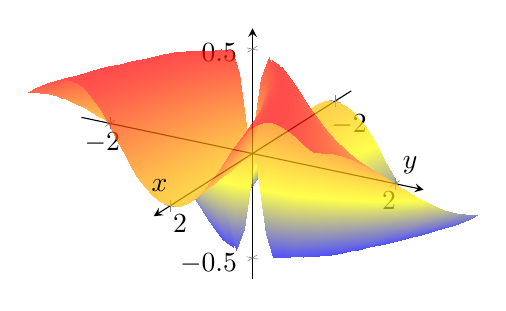
\begin{tikzpicture}
            \begin{axis}[
                view={120}{30}, % Angolazione della vista
                axis lines=center,
                xlabel={$x$},
                ylabel={$y$},
                domain=-2:2,
                y domain=-2:2,
                samples=40,
                samples y=40,
                enlargelimits=true,
                colormap/hot
            ]
                \addplot3[
                    surf,
                    shader=interp,
                    opacity=0.7,
                ]
                {x*y^2/(x^2 + y^4)};            
            \end{axis}
        \end{tikzpicture}
        \hspace{1cm}
        % Secondo grafico: altra vista
        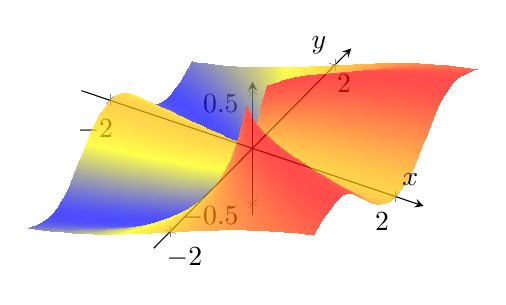
\begin{tikzpicture}
            \begin{axis}[
                view={30}{60}, % Angolazione alternativa della vista
                axis lines=center,
                xlabel={$x$},
                ylabel={$y$},
                domain=-2:2,
                y domain=-2:2,
                samples=40,
                samples y=40,
                enlargelimits=true,
                colormap/hot
            ]
                \addplot3[
                    surf,
                    shader=interp,
                    opacity=0.7,
                ]
                {x*y^2/(x^2 + y^4)};
            \end{axis}
        \end{tikzpicture}
    \end{center}

    Osserviamo innanzitutto il comportamento lungo ogni retta passante per \((0,0)\). Poniamo \(y=mx\) con \(m\in\mathbb{R}\). Sostituendo nella funzione otteniamo:
    \[
    f(x,mx)=\frac{x\,(mx)^2}{x^2+(mx)^4}=\frac{m^2 x^3}{x^2(1+m^4 x^2)}=\frac{m^2 x}{1+m^4 x^2}\,.
    \]
    Quindi, calcolando il limite per \(x\to0\), si ha:
    \[
    \lim_{x\to0} f(x,mx)=\lim_{x\to0}\frac{m^2 x}{1+m^4 x^2}=0\,.
    \]
    Pertanto, lungo ogni retta \(y=mx\) il limite risulta essere \(0\).

    Tuttavia, se consideriamo una curva diversa, per esempio la curva \(y=\sqrt{x}\) (che passa per \((0,0)\)), abbiamo:
    \[
    f\Bigl(x,\sqrt{x}\Bigr)=\frac{x\,( \sqrt{x})^2}{x^2+ (\sqrt{x})^4}
    =\frac{x\cdot x}{x^2+x^2}
    =\frac{x^2}{2x^2}=\frac{1}{2}\,.
    \]
    Il limite lungo la curva \(y=\sqrt{x}\) è quindi \(\frac{1}{2}\), diverso dal limite lungo le rette.

    Essendo il limite lungo differenti curve passanti per \((0,0)\) diverso (0 lungo le rette e \(1/2\) lungo \(y=\sqrt{x}\)), possiamo concludere che
    \[
    \nexists\,\lim_{(x,y)\to(0,0)} \frac{xy^2}{x^2+y^4}\,.
    \]
\end{exmp}

\vspace{10pt}

\begin{bxthm}
\begin{thm}
    Siano \[\lim_{(x,y)\to(x_0,y_0)}f(x,y)=l\in\overline{\mathbb{R}}\] e 
    \[\tau :I\subseteq\mathbb{R}\to\mathbb{R}\]
    una funzione continua definita in un intervallo $I$ contenente $y_0$ tale che 
    \begin{enumerate}
        \item $\tau(y_0)=x_0$, e 
        \item $\forall\, y\in I\setminus\{y_0\},\;(\tau(y),y)\in A$.
    \end{enumerate}
    Allora 
    \[\lim_{y\to y_0}f(\tau(y),y)=l.\]
\end{thm}
\end{bxthm}

\vspace{10pt}

\section{Calcolo dei limiti in due variabili}

\vspace{10pt}

% Calcolo del limite di una funzione di due variabili mediante coordinate polari

Siano $f:A\subseteq\mathbb{R}^2\to\mathbb{R}$ e $(x_0,y_0)\in\mathcal{D}(A)$.
L'obiettivo è calcolare il limite
\[
\lim_{(x,y) \to (x_0,y_0)} f(x,y).
\]

Per facilitare tale analisi si introduce un opportuno cambio di variabili mediante coordinate polari centrate in \((x_0,y_0)\). In particolare, si considerano le trasformazioni
\[
\begin{cases}
x = x_0 + \rho\cos\theta, \\[1mm]
y = y_0 + \rho\sin\theta,
\end{cases}
\]
dove \(\rho\in[0,+\infty[\) rappresenta la distanza tra il punto \((x,y)\) e il centro \((x_0,y_0)\), mentre \(\theta\in[0,2\pi]\) è l'angolo polare. 
In particolare, per definizione vale
\[
\rho = \sqrt{(x-x_0)^2 + (y-y_0)^2}.
\]

Sostituendo le relazioni precedenti nella funzione \(f\), definiamo la funzione trasformata in coordinate polari
\[
F(\rho,\theta) = f\bigl(x_0+\rho\cos\theta,\;y_0+\rho\sin\theta\bigr).
\]

Il dominio \(A^\star\) di $F(\rho,\theta)$ è ottenuto trasformando il dominio \(A\) in coordinate polari. 
In simboli:
\[A^\star=\{(\rho,\theta)\,:\;(x_0+\rho\cos\theta,y_0+\rho\sin\theta)\in A\}.\]

In questo modo, lo studio del limite di \(f\) per \((x,y)\to(x_0,y_0)\) si riduce all'analisi del comportamento di \(F(\rho,\theta)\) per \(\rho \to 0\) (con eventuale analisi uniforme rispetto al parametro \(\theta\)).

\vspace{10pt}

\begin{exmp}
    Siano 
    \[f:A=\mathbb{R}^2\setminus\{(0,0)\}\to\mathbb{R},\quad (x,y)\mapsto \dfrac{xy^3}{x^2+y^2}\] 
    e \((x_0,y_0)=(0,0)\).
    Vogliamo calcolare il limite di \(f\) per \((x,y)\to(0,0)\) mediante coordinate polari.
    Dalle ipotesi segue che
    \[\begin{cases}
        x=p\cos\theta\\
        y=p\sin\theta
    \end{cases}\quad \land\quad\rho=\sqrt{x^2+y^2}\]    
    \[F(\rho,\theta)=\dfrac{\rho\cos\theta\rho^3\sin^3\theta}{\rho^2\cos^2\theta+\rho^2\sin^2\theta}=\dfrac{\rho^4\cos\theta\sin^3\theta}{\rho^2(\cos^2\theta+\sin^2\theta)}=\dfrac{\rho^4\cos\theta\sin^3\theta}{\rho^2}=\rho^2\cos\theta\sin^3\theta\]
    $F$ è definita in 
    \[A^*=\{(\rho,\theta)\in[0,+\infty[\times[0,2\pi]\,:\;(\rho\cos\theta,\rho\sin\theta)\in A\}.\]
\end{exmp}

\vspace{10pt}

\begin{exmp}
    Sia \[C=\{(x,y)\in\mathbb{R}^2\,:\;\sqrt{x^2+y^2}\leq r\}\]
    il cerchio di centro \((0,0)\) e raggio \(r\).
    Traducendo in coordinate polari, otteniamo:
    \[C^\star=\{(\rho,\theta)\in[0,+\infty[\times[0,2\pi]\,:\;\sqrt{\rho^2\cos^2\theta+\rho^2\sin^2\theta}\leq r\}\]
    la condizione $\sqrt{\rho^2\cos^2\theta+\rho^2\sin^2\theta}\leq r$ si traduce in $\rho\leq r$.
    Pertanto, il cerchio in coordinate polari è rappresentato dal prodotto cartesiano:
    \[C^\star=[0,r]\times[0,2\pi]\]
\end{exmp}

\vspace{10pt}

Fissato $\theta\in[0,2\pi]$, definiamo la funzione $\varphi_\theta(\rho)=F(\rho,\theta)$, che rappresenta la funzione \(F\) lungo la semiretta con origine in \((0,0)\) e angolo \(\theta\).
La funzione \(\varphi_\theta\) è definita in 
\[A_\theta=\{\rho\in[0,+\infty[\;:\;(\rho,\theta)\in A^*\}.\]
Vogliamo che $A_\theta$ abbia $0$ come punto di accumulazione, perchè altrimenti non ha senso calcolare il limite \(\lim_{\rho\to0}\varphi_\theta(\rho)\).
Supponiamo come ipotesi che 
\[\exists\,C\in\mathcal{C}_{(x_0,y_0)}\,:\;C\setminus\{(x_0,y_0)\}\subseteq A.\]
Sia $r$ il raggio di $C$ e $\overline{C}=C\setminus\{(x_0,y_0)\}$.
Traducendo $\overline{C}$ in coordinate polari, otteniamo l'insieme 
\[\overline{C^\star}=]0,r]\times[0,2\pi]\subseteq A^\star\]
Poniamo $\rho\neq 0$ perchè il punto $(x_0,y_0)$ è escluso. Essendo inoltre $\sin\theta$ e $\cos\theta$ periodiche, se ci trovassimo a lavorare sugli assi, dovremo escludere altri punti insieme a $(x_0,y_0)$.

\vspace{10pt}

\begin{bxthm}
\begin{prop}
    Sia $A\subseteq\mathbb{R}^2$ tale che esiste un cerchio $C$ di centro $(x_0,y_0)$ e raggio $r>0$ con $C\setminus\{(x_0,y_0)\}\subseteq A$. 
    Allora per ogni $\theta\in[0,2\pi]$, l'intervallo $]0,r]$ è contenuto in $A_\theta$ e quindi $0$ è un punto di accumulazione per $A_\theta$.
\end{prop}
\end{bxthm}
\begin{proof}
    Fissiamo $\theta\in[0,2\pi]$ arbitrario. 
    Sia $\rho\in]0,r]$. Dobbiamo dimostrare che $\rho\in A_\theta$.
    
    Per definizione di $A_\theta$, questo equivale a dimostrare che $(\rho,\theta)\in A^*$.
    
    Per la definizione di $A^*$, questo significa dimostrare che il punto $(x_0+\rho\cos\theta,y_0+\rho\sin\theta)$ appartiene ad $A$.

    Osserviamo che:
    \begin{itemize}
        \item Il punto $(x_0+\rho\cos\theta,y_0+\rho\sin\theta)$ appartiene a $C\setminus\{(x_0,y_0)\}$ perché:
        \begin{itemize}
            \item La sua distanza da $(x_0,y_0)$ è $\rho\leq r$
            \item È diverso da $(x_0,y_0)$ perché $\rho>0$
        \end{itemize}
        \item Per ipotesi $C\setminus\{(x_0,y_0)\}\subseteq A$
    \end{itemize}

    Quindi $(x_0+\rho\cos\theta,y_0+\rho\sin\theta)\in A$, che implica $(\rho,\theta)\in A^*$ e di conseguenza $\rho\in A_\theta$.

    Avendo dimostrato che $]0,r]\subseteq A_\theta$, ne segue immediatamente che $0$ è un punto di accumulazione per $A_\theta$.
\end{proof}
\textbf{Dimostrazione originaria da rivedere}
% \begin{proof}
%     Sia $\theta\in[0,2\pi]$. Se $0<\rho\leq r, (\rho,\theta)\in\overline{C}\implies (x_0+p\cos\theta,y_0+\rho\sin\theta)\in\overline{C}\subseteq A\implies (\rho,\theta)\in A^*\implies \rho\in A_\theta$
% \end{proof}

% \vspace{10pt}
% 
% Posto
% \[\left(\begin{matrix}
%     x-x_0=\rho\cos\theta\\
%     y-y_0=\rho\sin\theta\\
% \end{matrix}\right),\]
% avremo che
% \[\rho\to0\implies\begin{cases}
%     x - x_0\to 0\\
%     y - y_0\to 0\\
% \end{cases}\implies\begin{cases}
%     x\to x_0\\
%     y\to y_0\\
% \end{cases}.\]

\vspace{10pt}

Poichè $0\in\mathcal{D}(A_\theta)$, ha senso fare $\lim_{\rho\to0}\varphi_\theta(\rho)$. 
Ma cosa vuol dire che 
\[\forall\,\theta\in[0,2\pi],\; \lim_{\rho\to0}\varphi_\theta(\rho)=l\in\mathbb{R}\;?\]
Vuol dire che 
\[\forall\,\varepsilon>0,\;\forall\,\theta\in[0,2\pi],\;\exists\,\delta>0\;(\delta\leq r)\,:\; 0<\rho<\delta\implies|\varphi_\theta(\rho)-l|<\varepsilon.\]

\vspace{10pt}

\paragraph{Limite uniforme}
\begin{bxthm}
\begin{defn}
Si dice che $\lim_{\rho\to0}\phi_\theta(\rho)=l\in\mathbb{R}$ è \textbf{uniforme} rispetto a $\theta$ se 
\[\forall\,\theta\in[0,2\pi],\;\forall\,\varepsilon>0,\;\exists\,\delta>0\,:\quad 0<\rho<\delta\implies|\varphi_\theta(\rho)-l|<\varepsilon.\quad\]
\end{defn}
\end{bxthm}

\vspace{10pt}

\begin{note}
Quando scriviamo che $\lim_{\rho\to0}F(\rho,\theta)=l$ è uniforme rispetto a $\theta$, stiamo parlando di $\varphi_\theta$, infatti è il limite di una sola variabile $\rho$.
\end{note}

\vspace{10pt}

\paragraph{Limite infinito uniforme}
\begin{bxthm}
\begin{defn}
    Si dice che $\lim_{\rho\to0}F(\rho,\theta)=+\infty$ è uniforme rispetto a $\theta$ se
    \[\forall\,\theta\in[0,2\pi],\;\forall\, M>0,\;\exists\,\delta>0\, :\; 0<\rho<\delta\implies F(\rho,\theta)\geq M.\]
    Allo stesso modo abbiamo che $\lim_{\rho\to0}F(\rho,\theta)=-\infty$ è uniforme rispetto a $\theta$ se
    \[\forall\,\theta\in[0,2\pi],\;\forall\, M<0,\;\exists\,\delta>0\, :\; 0<\rho<\delta\implies F(\rho,\theta)\leq M.\]
\end{defn}
\end{bxthm}

\vspace{10pt}

\paragraph{Teorema sul calcolo dei limiti}
\begin{bxthm}
\begin{thm}
    Siano $f:A\subseteq\mathbb{R}^2\to\mathbb{R}$, $(x_0,y_0)\in\mathcal{D}(A)$, e supponiamo che
    \[\exists\,C\in\mathcal{C}_{(x_0,y_0)}\,:\;C\setminus\{(x_0,y_0)\}\subseteq A.\]
    Allora \[\lim_{(x,y)\to(x_0,y_0)}f(x,y)=l\in\mathbb{R}\iff \lim_{\rho\to0}F(\rho,\theta)=l\textup{ è uniforme rispetto a }\theta.\]
\end{thm}
\end{bxthm}
\begin{proof}
    Dimostriamo l'equivalenza per $l\in\mathbb{R}$ (il caso $l=\pm\infty$ si dimostra in modo analogo).

    \begin{itemize}
        \item[$\implies$] Supponiamo che esista $\lim\limits_{(x,y)\to(x_0,y_0)}f(x,y)=l$. Per definizione di limite, questo significa che:
        \[\forall\,\varepsilon>0,\;\exists\,\delta>0\,:\;\forall\,(x,y)\in A,\quad 0<\|(x,y)-(x_0,y_0)\|<\delta\implies|f(x,y)-l|<\varepsilon.\]
        
        Dobbiamo dimostrare che il limite in coordinate polari è uniforme rispetto a $\theta$, ovvero:
        \[\forall\,\theta\in[0,2\pi],\;\forall\,\varepsilon>0,\; \exists\,\delta>0\;(\delta\leq r)\,:\quad 0<\rho<\delta\implies |F(\rho,\theta)-l|<\varepsilon.\]
        
        Fissiamo $\varepsilon>0$ e sia $\delta>0$ come nell'ipotesi. Consideriamo un punto arbitrario in coordinate polari con $0<\rho<\delta$ e $\theta\in[0,2\pi]$.
        Tale punto corrisponde in coordinate cartesiane a:
        \[\begin{cases}
            x=x_0+\rho\cos\theta\\
            y=y_0+\rho\sin\theta    
        \end{cases}\]
        
        Osserviamo che:
        \begin{itemize}
            \item $(x,y)\in A$ poiché $(\rho,\theta)\in A^*$ 
            \item La distanza di $(x,y)$ da $(x_0,y_0)$ è esattamente $\rho$:
            \[\|(x,y)-(x_0,y_0)\|=\sqrt{(x-x_0)^2+(y-y_0)^2}=\rho\]
        \end{itemize}
        
        Poiché $0<\rho<\delta$, le ipotesi del limite in coordinate cartesiane sono soddisfatte, quindi:
        \[|f(x,y)-l|<\varepsilon\]
        
        Ma $f(x,y)=F(\rho,\theta)$ in coordinate polari, quindi:
        \[|F(\rho,\theta)-l|<\varepsilon\]
        
        Questo prova l'uniformità del limite rispetto a $\theta$.

        \item[$\impliedby$] Supponiamo ora che il limite in coordinate polari sia uniforme, ovvero:
        \[\forall\,\varepsilon>0,\;\exists\,\delta>0\;(\delta\leq r)\,:\;\forall\,\theta\in[0,2\pi],\quad 0<\rho<\delta\implies|F(\rho,\theta)-l|<\varepsilon\]
        
        Dobbiamo dimostrare che esiste il limite in coordinate cartesiane.
        
        Sia $\varepsilon>0$ e sia $\delta>0$ come nell'ipotesi di uniformità. Consideriamo un punto $(x,y)\in A$ tale che $0<\|(x,y)-(x_0,y_0)\|<\delta$.
        
        Passando alle coordinate polari di questo punto:
        \begin{itemize}
            \item $\rho=\|(x,y)-(x_0,y_0)\|$ quindi $0<\rho<\delta$
            \item Esiste $\theta\in[0,2\pi]$ tale che:
            \[\begin{cases}
                x=x_0+\rho\cos\theta\\
                y=y_0+\rho\sin\theta
            \end{cases}\]
        \end{itemize}
        
        Per l'ipotesi di uniformità:
        \[|F(\rho,\theta)-l|<\varepsilon\]
        
        Tornando alle coordinate cartesiane:
        \[|f(x,y)-l|<\varepsilon\]
        
        Questo prova l'esistenza del limite in coordinate cartesiane.
    \end{itemize}
\end{proof}

\vspace{10pt}

\begin{exmp}
Calcoliamo il seguente limite:
\[
\lim_{(x,y)\to(0,0)}(x^2+y^2)e^{\sqrt{x^2+y^2}}
\]
Utilizziamo le coordinate polari:
\[
\begin{cases}
    x = \rho\cos\theta \\
    y = \rho\sin\theta
\end{cases}
\quad\text{con}\quad \rho = \sqrt{x^2+y^2}
\]
Sostituendo otteniamo:
\[
\begin{aligned}
    F(\rho,\theta) &= (\rho^2\cos^2\theta + \rho^2\sin^2\theta)e^{\rho} \\
    &= \rho^2(\cos^2\theta + \sin^2\theta)e^{\rho} \\
    &= \rho^2e^{\rho}
\end{aligned}
\]
Osserviamo che $F(\rho,\theta)$ non dipende da $\theta$, quindi:
\[
\lim_{\rho\to0}F(\rho,\theta) = \lim_{\rho\to0}\rho^2e^{\rho} = 0
\]
Poiché la funzione non dipende da $\theta$, il limite è uniforme rispetto a $\theta$ e dunque possiamo concludere che:
\[
\lim_{(x,y)\to(0,0)}(x^2+y^2)e^{\sqrt{x^2+y^2}} = 0
\]
\end{exmp}

\vspace{10pt}

Per calcolare $\lim_{\rho\to0}F(\rho,\theta)$, serve che per ogni $\theta\in[0,2\pi]$, $A_\theta$ abbia $0$ come punto di accumulazione.
Supponiamo che $\forall\,\theta\in[0,2\pi]$ $A_\theta\neq\emptyset$ oppure $0\notin\mathcal{D(A)}$.

\vspace{10pt}

\paragraph{$\theta$ ammissibile}
\begin{bxthm}
\begin{defn}
    Si dice che $\theta\in[0,2\pi]$ è \textbf{ammissibile} se $0\in\mathcal{D}(A_\theta)$.
\end{defn}
\end{bxthm}

\vspace{10pt}

\begin{note}
    \[\varphi_\theta(\rho)=F(\rho,\theta)=f(x_0+\rho\cos\theta,y_0+\rho\sin\theta)\to f(x_0,y_0)\textup{ per }\rho\to0.\]
\end{note}

\vspace{10pt}

\begin{exmp}
    
\end{exmp}

\vspace{10pt}

Sia \[\lim_{\rho\to0}F(\rho,\theta)=l\in\mathbb{R}.\] Allora \[\phi(\rho)=\sup\{|<F(\rho,\theta)-l|:\theta\in[0,2\pi]\}.\]

\begin{bxthm}
\begin{thm}
    $\lim_{\rho\to0}F(\rho,\theta)=l\in\mathbb{R}$ uniformemente rispetto a $\theta \iff \lim_{\rho\to0}\phi(\rho)=0$.
\end{thm}
\end{bxthm}
\begin{proof}
    Per ipotesi, \[\forall\varepsilon>0,\exists\delta>0:0<\rho<\delta\implies|F(\rho,\theta)-l|<\frac{\varepsilon}{2}\;\forall\theta\]
    \[\sup|F(\rho,\theta)-l| (=\phi(\rho))\leq\dfrac{\varepsilon}{2}<\varepsilon\]
    \[\phi(\rho)\geq0\quad \phi(\rho)=|\phi(\rho)|\]
    \[\forall\varepsilon>0,\exists\delta>0: se 0<\rho<\delta, |\phi(\rho)|<\varepsilon\implies \lim_{\rho\to0}\phi(\rho)=0.\]
    $\impliedby$
    Per ipotesi, \[\forall\varepsilon>0,\exists\delta>0: se 0<\rho<\delta, |\phi(\rho)|<\varepsilon.\]
    \[\phi(\rho)<\varepsilon.\]
    Finire dimostrazione.
\end{proof}
\[F(\rho,\theta)=\dfrac{\rho\cos\theta\rho^3\sin^2\theta}{\rho^2}=\rho^2\cos\theta\sin^3\theta. \]
\[\lim_{\rho\to0}F(\rho,\theta)=0.\]

\begin{bxthm}
\begin{cor}
    \[\lim_{\rho\to0}F(\rho,\theta)=l\in\mathbb{R}\] uniformemente rispetto a $\theta \iff \exists$ una funzione \[\psi(p):\lim_{\rho\to0}\psi(\rho)=0\] e \[|F(\rho,\theta)-l|\leq\psi(\rho)\forall\theta\]
\end{cor}
\end{bxthm}
\begin{proof}
    $\implies$ Per il teorema precedente, $\lim_{\rho\to0}\phi(\rho)=0$. Per definizione di $\phi$, \[|F(\rho,\theta)-l|\leq\phi(\rho)\forall\theta\]
    $\psi=\phi$ . $\psi \exists$ ed è la funzione $\phi$
    $\impliedby$ \[|F(\rho,\theta)-l|\leq\psi(\rho)\forall\theta\implies 0\leq\phi(\rho)\leq\psi(\rho)\forall\theta\implies\lim_{\rho\to0}\phi(\rho)=0\] per il teorema dei carabinieri.
\end{proof}

Segue esempio che devi fare

\[\lim_{\rho\to0}F(\rho,\theta)=+\infty \quad h(\rho)=\inf\{F(\rho,\theta):\theta\}\]
\begin{bxthm}
\begin{thm}
    $\lim_{\rho\to0}F(\rho,\theta)=+\infty$ uniformemente rispetto a $\theta \iff \lim_{\rho\to0}h(\rho)=+\infty$
\end{thm}
\end{bxthm}
\begin{bxthm}
\begin{cor}
    $\lim_{\rho\to0}F(\rho,\theta)=+\infty$ uniformemente rispetto a $\theta \iff \exists$ una funzione $k(\rho)$ : $\lim_{\rho\to0}k(\rho)=+\infty$ e $F(\rho,\theta)\geq k(\rho)\forall\theta$.
\end{cor}
\end{bxthm}

Ad esempio 
\[\lim_{(x,y)\to(0,0)}\dfrac{1+x^2y^2}{(x^2+y^2)^2} A=\mathbb{R}^2\setminus\{(0,0)\}\]
$F(\rho,\theta)=\dfrac{1+\rho^2\cos^2\theta\sin^2\theta}{\rho^2}$
$\lim_{\rho\to0}F(\rho,\theta)=+\infty$
\[1+\rho^4\cos^2\theta\sin^2\theta\geq1\]
\[F(\rho,\theta)\geq\dfrac{1}{\rho^4}\forall\theta\]
$\dots$


\[\lim_{\rho\to0}F(\rho,\theta)=-\infty\quad\quad t(\rho)=\sup\{F(\rho,\theta):\theta\}\]
\begin{bxthm}
\begin{thm}
    $\lim_{\rho\to0}F(\rho,\theta)=-\infty$ uniformemente rispetto a $\theta \iff \lim_{\rho\to0}t(\rho)=-\infty$.
\end{thm}
\end{bxthm}
\begin{bxthm}
\begin{cor}
    $\lim_{\rho\to0}F(\rho,\theta)=-\infty$ uniformemente rispetto a $\theta \iff \exists$ una funzione $\theta(\rho):\lim_{\rho\to0}\theta(\rho)=-\infty$ e $F(\rho,\theta)\leq\theta(\rho)\forall\theta$
\end{cor}
\end{bxthm}

Se $\exists 2$ rette e $2$ curve passanti per $(x_0,y_0)$ lungo le quali $f$ tende a limiti distinti, $\lim_{(x,y)\to(x_0,y_0)}f(x,y)\nexists$.
Se $\exists$ una retta e una curva passante per $(x_0,y_0)$ lungo la quale $f$ non ha limite, $\lim_{(x,y)\to(x_0,y_0)}f(x,y)\nexists$

\begin{xca}
Calcolare i seguenti limiti:
\[\lim_{(x,y)\to(0,0)}\dfrac{x^2y^2}{x^2+y^2}\]
\[\lim_{(x,y)\to(0,0)}(x^2-y^2)e^{\sqrt{x^2+y^2}}\]
\[\lim_{(x,y)\to(0,0)}\dfrac{x^2+2y^2}{(x^2+y^2)^4}\]
\end{xca}








\end{document}
